\documentclass[lettersize,journal]{IEEEtran}

% Math
\usepackage{amsmath,amssymb,amsfonts,amsthm}
\newtheorem{theorem}{Theorem}
\newtheorem{lemma}{Lemma}

% Figures and floats
\usepackage{graphicx}
\usepackage{subcaption}
\usepackage{stfloats}
% \usepackage{subcaption}
% Tables and arrays
\usepackage{array}
\usepackage{booktabs}
\usepackage{multirow}

% Algorithms
\usepackage{algorithm}
\usepackage{algpseudocode}

% Text and symbols
\usepackage[T1]{fontenc}
\usepackage[utf8]{inputenc} %
\usepackage{textcomp}
\usepackage{xcolor}

% References and links
\usepackage{cite}
\usepackage{url}
\usepackage{hyperref}

% Optional utilities
\usepackage{verbatim}
\usepackage{nicefrac}
\usepackage{microtype}
\newcommand{\good}[1]{{\color{green!50!black}$\downarrow$#1}}
\newcommand{\bad}[1]{{\color{red!70!black}$\uparrow$#1}}

\newcommand{\hfj}[1]{\textcolor{red}{#1}}

\hyphenation{op-tical net-works semi-conduc-tor IEEE-Xplore}


\begin{document}

\title{DiBS: Diffusion-Informed Branch Selection}

%\IEEEauthorrefmark{1} \IEEEauthorrefmark{2} \IEEEauthorrefmark{3}

\author{\IEEEauthorblockN{
Bo Liu,~\IEEEmembership{Graduate Student Member, IEEE},
Yuan Xie,
Yuan Gao,
XiaoLong Luo, \\
Peng Ye,
Tao Chen,~\IEEEmembership{Senior Member,~IEEE}, and
Fujun Han,~\IEEEmembership{Member,~IEEE}
}
% \IEEEauthorblockA{\IEEEauthorrefmark{1}School of Electrical and Computer Engineering,
% Georgia Institute of Technology, Atlanta, GA 30332 USA}
% \IEEEauthorblockA{\IEEEauthorrefmark{2}Twentieth Century Fox, Springfield, USA}
% \IEEEauthorblockA{\IEEEauthorrefmark{3}Starfleet Academy, San Francisco, CA 96678 USA}
% \IEEEauthorblockA{\IEEEauthorrefmark{4}Tyrell Inc., 123 Replicant Street, Los Angeles, CA 90210 USA}% <-this % stops an unwanted space
\thanks{
%This work was supported by the National Natural Science Foundation of
%China. (\textit{Corresponding author: Fujun Han}.) \\
This work was supported in part by The Chinese University of Hong Kong, Shenzhen, and the Shanghai Artificial Intelligence Laboratory. The authors would like to thank those who provided essential support and assistance during the development of this research. (\textit{Corresponding author: Fujun Han}) \\
\hspace*{0.72em} Bo Liu is with the School of Mathematics, Jilin University, Changchun 130012, China (liubo1022@mails.jlu.edu.cn). \\
\hspace*{0.6em} Yuan Xie and Yuan Gao are with the School of Data Science, The Chinese University of Hong Kong, Shenzhen, Shenzhen 518171, China (224040374@link.cuhk.edu.cn, 225080020@link.cuhk.edu.cn).\\
\hspace*{1.05em} Xiaolong Luo is with the Business School, Southwest University, Chongqing 402460, China (luoxl0306@163.com). \\
\hspace*{1.05em} Peng Ye is with the Multimedia Laboratory, The Chinese University of Hong Kong, Hong Kong 999077, China, also with the Shanghai Artificial Intelligence Laboratory, Shanghai 200032, China (yepeng@pjlab.org.cn). \\
\hspace*{1.05em} Tao Chen is with the School of Information Science and Technology, Fudan University, Shanghai 200433, China (e-mail: eetchen@fudan.edu.cn). \\
\hspace*{1.06em} Fujun Han is with the School of Data Science, The Chinese University of Hong Kong, Shenzhen, Shenzhen 518171, China (hanfujun@cuhk.edu.cn).
}
}

% \author{%
% 	Bo Liu$^1$,
% 	Yuan Xie$^{2}$,
% 	Yuan Gao$^{2}$,
% 	Fujun Han$^{2}$\thanks{Corresponding Author} \\
% 	%Department of Computer Science\\
% 	$^1$ School of Mathematics, Jilin University \\
% 	$^2$ School of Data Science, The Chinese University of Hong Kong, ShenZhen \\
% 	%Pittsburgh, PA 15213 \\
% 	\texttt{liubo1022@mails.jlu.edu.cn, hanfujun@cuhk.edu.cn} \\
% }
% The paper headers
\markboth{IEEE Transactions on Knowledge and Data Engineering}%
{Shell \MakeLowercase{\textit{et al.}}: A Sample Article Using IEEEtran.cls for IEEE Journals}

% Remember, if you use this you must call \IEEEpubidadjcol in the second
% column for its text to clear the IEEEpubid mark.

\maketitle

\begin{abstract}

Sudoku is a representative constraint satisfaction problem that requires global structural reasoning under strict discrete constraints.
% Recent deep learning solvers can capture useful global patterns, but they are not guaranteed to provide results fitting constraints when used to generate solutions directly.
% Classical symbolic solvers, in contrast, are complete, but their search is guided mostly by local propagation and handcrafted heuristics, making hard instances vulnerable to long-tail behavior caused by wrong early branch-ordering decisions.
% The existing approaches to Sudoku solving suffer from two complementary limitations: learning-based solvers lack hard correctness guarantees despite their ability to capture global patterns, whereas complete symbolic solvers are still prone to long-tail search because their branching decisions are mainly guided by local heuristics.
The existing works of solving Sudoku mainly focus on two dominant approaches, \textit{i.e.}, traditional heuristic and deep learning solver. However, they suffer from two complementary limitations: learning-based solvers lack hard correctness guarantees, while complete symbolic solvers are still prone to long-tail search.
To address these shortcomings, a novel diffusion model-guided approach, termed as \textbf{DiBS}, is proposed for branch selection search process.
% we propose a novel approach branch Selection by diffusion model guided, termed as \textbf{DiBS}.
% Specifically, our DiBS augments a complete symbolic solver while leaving propagation, variable selection, and completeness unchanged. in binary branching states, DiBS queries a diffusion model under the current partial assignment and uses its conditional preferences, together with a lightweight consistency signal, to rank candidate values more effectively.
Specifically, DiBS keeps the symbolic solver complete and uses the diffusion model as a branch-ordering guide. The core method is ranking candidate values under the current partial assignment and lightweight consistency signal.
Furthermore, we provide an in-depth theoretical proof to reveal how it works and why it works.
% The analysis shows that the expected cost of search decomposes into solution-path cost, model-inference overhead, and posterior-weighted wrong-subtree cost, clarifying how model capability determines whether search savings can amortize inference time.
Experiments on the most challenging Sudoku benchmarks: Royle's 17-clue, show that our DiBS substantially reduces search cost relative to strong symbolic baselines, especially in nodes, backtracks, and long-tail percentiles. Besides, these results confirm that learned global guidance is particularly effective on hard instances where branch-order mistakes are most expensive.
All codes and datasets are available at \url{https://github.com/shanxierdan/DiBS}.

\end{abstract}


\begin{IEEEkeywords}
Diffusion Model, Constraint Satisfaction Problem
\end{IEEEkeywords}

\section{Introduction}

\IEEEPARstart{S}{udoku} \hfj{is a well-known combinatorial puzzle, and it is often formulated as a constraint satisfaction problem (CSP).} Classical solvers for CSPs typically rely on depth-first backtracking, constraint propagation (CP), minimum remaining values (MRV) and consistency algorithms. These solvers are complete, meaning they will find a solution if one exists and prove unsatisfiability otherwise. \hfj{However, in difficult cases, the performance is usually determined by two parts, \textit{i.e.},
constraint propagation and the structure of the search tree.} A few early wrong branching decisions can lead to enormous failing subtrees, which only reveal contradictions deep into the search process. This phenomenon results in long-tail runtimes, particularly in algorithms designed to challenge search solvers \cite{mackworth1977consistency, haralick1980increasing, regin1994filtering, simonis2005sudoku}.

\begin{figure}[t]
\centering
\includegraphics[width=0.95\linewidth]{figures/intro1.png}
% \caption{Overview of the three approaches, DiBS is a new paradigm compared with Traditional heuristic solver and other Deep Learning solvers.}
\caption{The comparison of three different solver paradigms. We can find that our DiBS is a new paradigm compared with Traditional heuristic solvers and other Deep Learning solvers.}
\label{fig:solver_methods}
\end{figure}

\hfj{In recent years, some learned models, \textit{e.g.}, recurrent relational networks (RRNs) and differentiable solvers (SATNet) have been explored as a means to guide search processes. These models have demonstrated the potential to capture the global structure of problems like Sudoku \cite{palm2018recurrent, wang2019satnet}. While these approaches present promising performance on directly generating solutions, they often adopt an end-to-end approach and bypass the exact search mechanisms of classical solvers. However, this shift raises a basic and important question: %\textit{Is it possible to use generative models not to replace symbolic reasoning, but to guide it in a way that improves efficiency without sacrificing completeness?}
\textit{Is it possible to use generative models to guide it in a way that improves efficiency without sacrificing completeness?}}

\hfj{To answer this question, we carefully review and investigate the existing promising works and find that recent diffusion models work for discrete domains, \textit{e.g.}, structured denoising diffusion models (D3PMs) and graph-based diffusion solvers (GSDM), have extended the capabilities of generative models beyond image generation. Beises, these works also apply them to complex combinatorial problems, \textit{e.g.}, Sudoku and other CSPs \cite{ho2020denoising, austin2021structured, weilbach2023graphically}.} For Sudoku, this means a model can encode which candidate assignments are globally compatible with a partial grid, even when that compatibility is not exposed by local propagation alone. \hfj{However, most pure and combinatorial optimization diffusion models mainly focus on full-solution generation, yet they ignore offering guidance during the branch selection search process \cite{sun2023difusco, ye2025beyond}}, \textcolor{blue}{which will lead to xxxxx (two challenges in abstract!)}


\hfj{In this paper, we are dedicated to simultaneously solving the above-mentioned two challenges.} We argue that the value of learned models in exact solvers lies not in generating complete solutions, but in improving search by guiding branch ordering at high-leverage decision points.
\hfj{Different from previous works, \textit{e.g.}, the learned branching in combinatorial optimization \cite{khalil2016learning, gasse2019exact} and model-based planning with learned models \cite{schrittwieser2020muzero, janner2022diffuser}, our goal is more specific. We use diffusion-model guidance only to rank candidate values within a complete CP+MRV procedure, rather than replace the solver or learn a full decision policy, thereby preserving propagation, variable selection, and completeness.} Specifically, If \(p_s\) denotes the probability of selecting the solution-leading branch first at state \(s\), and \(T(s_w)\) denotes the cost of exploring the failing subtree when the wrong branch is tried first, then the expected search reduction from better guidance scales with \(\Delta p_s \cdot T(s_w)\). This makes learned branch ordering especially valuable in the heavy-tail regime, where even a modest improvement in ranking accuracy can prevent a disproportionately large amount of wasted exploration. \hfj{Based on this principle, we propose \textbf{DiBS} (iffusion-Informed Branch Selection), a novel diffusion model-guided approach. As shown in Fig.~\ref{fig:solver_methods}, different from previous work, our DiBS is a new solver paradigm for the branch selection search process. DiBs injects diffusion-model preferences into exact symbolic Sudoku solving by reordering branches without pruning the search space. Rich experiments and comparisons on challenging Sudoku benchmarks denote that the proposed DiBs is effective and efficient, showing promising performance improvements in multiple metrics.}

In total, our contributions can be summarized as follows:
\begin{itemize}
    \item \textbf{Novel Paradigm.} \hfj{To the best of our knowledge, DiBS is the first attempt to apply a diffusion model to guide branch selection. xxxxxxx. Experiments in the hardest dataset show our method is stronger than heuristic baselines in search cost.} %The discussion further reveals the various aspects of our method.
    \item\textbf{Universal Theoretical Framework.} \hfj{We design probabilistic branch-ordering framework. xxxxxx. Our probabilistic framework can be generalized to branch-ordering policies.}
    % Our theory presents a probabilistic framework for not just DiBS, but all branch-ordering policies. It proves that selecting solution-leading branches earlier reduces search cost in proportion to the cost of failing subtrees and formalizes the optimal strategy. Our math explains DiBS's effectiveness and its ability to systematically approach the optimal solution, providing a foundation for future probabilistic branch-ordering methods.
    \item \textbf{Broader Principle.} \hfj{We xxxxxxx.}
    In branching-based solvers, learned global priors can be injected into local decision ordering without replacing the underlying solver or compromising its correctness. This principle provides a general approach for integrating generative guidance into structured discrete search methods. While DiBS is demonstrated on Sudoku, it has the potential to be extended to other CSPs and NP problems, suggesting a promising direction for future research.
\end{itemize}

\section{Related Work}

\subsection{From Generative Modeling to Diffusion-Based Structural Knowledge}

Generative modeling has evolved from latent-variable and adversarial formulations to large-scale conditional generation, and this evolution is relevant to our work because it suggests that generative objectives can induce nontrivial structural knowledge about data.
Early milestones such as variational autoencoders (VAEs) and generative adversarial networks (GANs) showed that neural models can learn useful latent representations and rich data distributions from raw observations \cite{kingma2013autoencoding,goodfellow2014gan}.
The Transformer further broadened the scope of generative modeling by enabling scalable sequence modeling with strong global context integration \cite{vaswani2017attention}.
Diffusion models have since become a particularly important family of generative models.
Starting from denoising diffusion probabilistic models (DDPMs), subsequent work introduced faster or more flexible variants such as DDIM, score-based diffusion via stochastic differential equations, latent diffusion, and transformer-based diffusion backbones, including DiT \cite{ho2020ddpm,song2020ddim,song2021sde,rombach2022ldm,peebles2023dit}.
These developments established diffusion as a general framework for learning high-dimensional structure, not only for image synthesis but also for conditional generation and controllable inference \cite{han2024ada,han2024mmid}.
A broader trend is that generative models are increasingly used to support understanding, planning, and decision-making rather than generation alone.
World models learn latent environment dynamics that can be exploited for planning and policy learning \cite{ha2018worldmodels,hafner2023dreamerv3}.
Diffusion-based planning methods similarly reinterpret denoising as iterative trajectory optimization \cite{janner2022planning}.
At larger scales, generative interactive environments and vision-language-action models suggest that generative objectives can capture semantic, causal, and action-relevant regularities that transfer to downstream control and reasoning tasks \cite{bruce2024genie,brohan2023rt2}.
These works motivate our central perspective: the value of a generative model may lie not only in its samples, but also in the structured prior knowledge it learns and can provide to another algorithmic system.

\subsection{Generative Models for Sudoku, Reasoning, and Planning}

Recent work has extended diffusion and related generative models from perceptual generation to discrete reasoning and structured completion tasks.
Discrete diffusion models such as D3PM explicitly adapt diffusion to categorical state spaces \cite{austin2021d3pm}, while later formulations further study continuous-time or masked variants for discrete domains \cite{campbell2022ctdd,kim2024tokenorder,garg2025learnedorder}.
These developments are especially relevant for Sudoku, where the state is discrete, globally constrained, and only partially observed.
Several works have used generative models directly on Sudoku or closely related reasoning settings.
Graphically Structured Diffusion Models (GSDM) encode sparse variable interactions and demonstrate effective conditional inference in structured problems including Sudoku-like settings \cite{weilbach2023gsdm}.
Dirichlet Diffusion Score Models (DDSM) show that conditional sampling with clamped clues can solve Sudoku without additional task-specific retraining \cite{avdeyev2023ddsm}.
Beyond Autoregression studies discrete diffusion as a general paradigm for complex reasoning and planning, reporting strong results on Sudoku and related tasks \cite{ye2025beyondar}.
Spatial Reasoning Models (SRMs) and recent studies on token ordering in masked diffusion further show that update order, uncertainty, and sequentialization can materially affect reasoning performance on structured puzzles \cite{wewer2025srm,kim2024tokenorder}.
Despite these advances, most of the above methods still treat Sudoku primarily as a generation or reconstruction problem: the model is expected to iteratively produce the full solution under partial observations.
Our work differs in objective and interface.
We do not use diffusion to replace search or to directly output the final board.
Instead, we use the diffusion model as a conditional prior that ranks candidate values inside a complete symbolic solver.
In this sense, we use generative knowledge to guide exact reasoning rather than to bypass it.

\subsection{Constraint Satisfaction, Exact Solving, and Learned Search Guidance}

Sudoku is a classical constraint satisfaction problem (CSP), and its exact solution methods are rooted in the broader literature on constraint programming.
Foundational work established core notions such as consistency, propagation, and search control \cite{mackworth1977consistency,haralick1980search,freuder1982sufficient}.
Subsequent research developed stronger propagation algorithms and global constraints, including influential work on arc consistency and AllDifferent filtering \cite{mohr1993ac6,regin1994alldiff}.
These ideas are now standard in textbooks and handbooks on CSP and CP \cite{apt2003principles,dechter2003constraint,rossi2006handbook,russell2010aima}.
Beyond puzzle solving, CSP and CP techniques have been applied to a wide range of real-world problems, including scheduling, air-traffic management, software verification, autonomous driving, and product configuration \cite{bartak2010survey,gotlieb2012tcas,benavides2010featuremodels}.
This broader application context matters for our work: it suggests that methods which preserve completeness and solver reliability while improving search efficiency can have value well beyond Sudoku itself.
Another closely related line of work concerns learned guidance for exact search.
In Sudoku specifically, recurrent relational networks and differentiable satisfiability layers show that neural systems can capture global constraints and relational structure \cite{palm2018rrn,wang2019satnet}.
However, such methods typically aim at direct solution prediction rather than improving a complete search procedure.
In optimization, learned branching policies have been used to guide branch-and-bound and related exact solvers, demonstrating that learned models can reduce search effort without replacing the symbolic backbone \cite{khalil2016l2branch,gasse2019exact,scavuzzo2022treemdp}.
Our method is closest in spirit to this final category.
Like learned branching, DiBS injects a learned prior into an exact solver while preserving correctness guarantees.
However, our setting and mechanism are different: we focus on complete CP-style solving for Sudoku/CSPs, and we use a diffusion model to guide value ordering at high-leverage branching states rather than learning variable selection alone.
This positions DiBS between two traditionally separate literatures: generative modeling as a source of global structural knowledge, and exact CSP solving as a source of soundness, completeness, and controllable search.

\begin{figure*}[t]
	\centering
	\includegraphics[width=0.98\textwidth]{figures/Tree.jpg}
        \caption{Search-behavior comparison between MRV and DiBS on a representative puzzle.
(a) Tree-structure visualization of the explored search space. Blue edges denote regular expansions and red edges highlight deep erroneous branches, which are the main source of wasted search.
(b) Depth profile of expanded nodes. Compared with MRV, DiBS avoids broad frontier growth and reduces the number of explored states, especially along deep erroneous branches.}
\label{fig:search_behavior}
\end{figure*}

\section{Preliminaries}
\label{sec:preliminaries}

\subsection{Sudoku and constraint satisfaction problems}
We view Sudoku as a special case of a constraint satisfaction problem (CSP). A CSP is specified by a triple
\[
\mathcal{P}=(V,\mathcal{D},\mathcal{C}),
\]
where $V$ is a finite set of variables, $\mathcal{D}=\{D_v\}_{v\in V}$ assigns each variable $v$ a finite domain $D_v$, and $\mathcal{C}$ is a set of constraints over subsets of variables.

In standard $9\times 9$ Sudoku, we take $V=\{1,\dots,81\}$, one variable per cell. Each variable $v\in V$ takes a value in $\{1,\dots,9\}$, so initially $D_v\subseteq\{1,\dots,9\}$, with the given clues encoded as singleton domains. We represent a partial grid by a partial assignment
\[
x:V\rightarrow \{0,1,\dots,9\},
\]
where $x(v)=0$ means that cell $v$ is unassigned, and $x(v)\in\{1,\dots,9\}$ is an assigned digit.

Sudoku constraints enforce that within every row, column, and $3\times 3$ block, all digits are distinct. For convenience we use pairwise inequality constraints. Let $N(v)\subseteq V$ denote the set of neighbors of $v$, namely all variables that share a row, a column, or a block with $v$ (excluding $v$ itself). Let
\[
A(x)=\{v\in V:\ x(v)\neq 0\}
\]
denote the set of assigned variables under a (partial) assignment $x$. Then feasibility of $x$ means that no two assigned neighboring cells share the same digit:
\[
x(u)\neq x(v)\qquad \forall\, v\in A(x),\ \forall\, u\in N(v)\cap A(x).
\]
A complete solution is an assignment $x^\star$ with $A(x^\star)=V$ that satisfies the constraints above.



\subsection{Discrete diffusion for Sudoku reasoning}

Our diffusion prior is instantiated using the discrete diffusion framework of \cite{ye2025beyond}, whose model is trained for complex reasoning and planning tasks including Sudoku. In their setting, a complete Sudoku solution is represented as a discrete token sequence
\[
x_0 \in \{1,\dots,9\}^{81},
\]
and training constructs corrupted versions \(x_t\) through an absorbing-state discrete noising process over timesteps \(t \in \{1,\dots,T\}\). Intuitively, more positions are masked or corrupted at larger \(t\), and the neural network is trained to recover the clean tokens from these partially corrupted views.

Formally, the model learns a reverse denoising distribution \(p_\theta(x_{t-1}\mid x_t)\) on top of a discrete forward corruption process \(q(x_t\mid x_{t-1})\). Rather than directly optimizing the full variational objective, \cite{ye2025beyond} show that for absorbing-state discrete diffusion, the denoising objective can be written as a weighted cross-entropy loss over corrupted tokens:
\begin{equation}
	\mathcal{L}_{\mathrm{DM}}
	=
	\mathbb{E}_{q(x_0)}
	\sum_{n=1}^{N}\sum_{t=1}^{T}
	w(t)\,
	\mathbb{E}_{q(x_t\mid x_0)}
	\,u(x_0,x_t,n;\theta),
	\label{eq:dm_loss}
\end{equation}
where \(N\) is the sequence length, \(w(t)\) is a timestep-dependent weight, and
\begin{equation}
	u(x_0,x_t,n;\theta)
	:=
	-\mathbf{1}[x_{t,n}\neq x_{0,n}]\, x_{0,n}^{\top}\log f_\theta(x_t)_n
	\label{eq:dm_token_loss}
\end{equation}
is the token-level cross-entropy loss for reconstructing the clean token at position \(n\). This objective trains the model to predict missing or corrupted digits from partially observed global contexts, which is especially suitable for Sudoku because the validity of one cell depends on long-range row, column, and block interactions.

In DiBS, we do not use this model as an end-to-end generator. Instead, we use the trained denoiser as a conditional prior over candidate digits under the current partial Sudoku state. Given a solver state \(s=(x,\{D_v\}_{v\in V})\), we encode the current partial assignment as a conditioning grid and query the model once to obtain per-cell logits over digits. These logits are then converted into candidate probabilities and used only for branch ordering inside a complete symbolic solver. This design preserves the completeness of CP-based search while importing the global pattern knowledge learned by the diffusion model.



\subsection{CP and MRV}

Our symbolic backbone is a standard complete solver based on constraint propagation (CP), depth-first backtracking, and Minimum Remaining Values (MRV)\cite{freuder1982sufficient}. At any point in the search, the solver maintains a state consisting of a partial assignment \(x\) together with current candidate domains \(\{D_v\}_{v\in V}\), where each \(D_v \subseteq \{1,\dots,9\}\) contains the digits still feasible for cell \(v\).

Constraint propagation (CP) is applied after every assignment. In Sudoku, assigning a digit to one cell immediately restricts all peer cells in the same row, column, and \(3\times 3\) block. Therefore, after setting \(x(v)=d\), CP removes \(d\) from the domains of all peers \(u\in N(v)\), and recursively applies any deterministic consequences of this update. More generally, CP shrinks domains by enforcing local consistency with respect to the Sudoku constraints before further branching. If propagation makes some domain empty, i.e., \(D_u=\varnothing\) for some unassigned variable \(u\), then the current partial assignment cannot be extended to a valid solution and the solver backtracks immediately. In this way, CP prunes infeasible branches early and reduces the effective search space.

When propagation alone cannot finish the puzzle, the solver branches on one unassigned variable. We use the widely adopted Minimum Remaining Values (MRV) heuristic, which selects a variable with the smallest remaining domain:
\begin{equation}
	v^\star \in \arg\min_{v:\,x(v)=0} |D_v|.
	\label{eq:mrv}
\end{equation}
The intuition is the standard fail-first principle: variables with fewer legal values are more constrained and are therefore more informative branching points. Once \(v^\star\) is selected, the solver tries values in \(D_{v^\star}\) one by one, each time invoking CP and then recursing. The solver remains complete as long as all candidates are eventually explored when needed. Consequently, changing only the value order for \(D_{v^\star}\) affects efficiency but never correctness.

\section{Method}
\label{sec:method}

\begin{figure*}[h]
	\centering
	\includegraphics[width=0.98\textwidth]{DiBS.png}
	\caption{Overall pipeline of the proposed \textbf{DiBS}. Starting from an incomplete Sudoku grid, the CP+MRV solver selects the next branching variable. At binary MRV states, the current partial assignment is represented as a masked grid and passed to a discrete diffusion model, which provides conditional preference scores for the candidate values. These scores are combined with a consistency penalty to determine the branch ordering. The solver then explores the preferred branch first, backtracks only when a contradiction is encountered, and repeats this procedure until the puzzle is solved.}
	\label{fig:overview}
\end{figure*}

\subsection{Motivation: diffusion as probabilistic branch guidance}
Complete backtracking Sudoku solvers spend most of their time exploring \emph{failing} subtrees caused by early wrong decisions.
On very hard instances (e.g., 17-clue puzzles), an incorrect branch often does not contradict immediately; instead, it fails only after deep propagation and many recursive calls.
Therefore, even without pruning any candidate, improving the order in
which branches are tried can substantially reduce the total
search cost and tail latency, as illustrated by the representative
search-behavior comparison in Fig.~\ref{fig:search_behavior}.

Diffusion models trained for Sudoku completion provide a probabilistic signal about which digit is more plausible for a given cell under a partial grid.
Rather than using the model to directly generate a full solution (which may violate hard constraints and requires resampling), we use it as a branch preference oracle inside a symbolic, complete solver.
To keep inference overhead amortized, we only query the model at a small subset of high-leverage decision points.

\subsection{Principle: How DiBS works for branch ordering}
As shown in Fig~\ref{fig:overview}, DiBS augments a standard complete solver with constraint propagation, MRV variable selection, and depth-first backtracking.
The key modification is that, at each branching decision, DiBS uses a trained diffusion model to order the candidate digits for the selected cell---it never prunes any candidate, thus preserving completeness.


Let $V$ be the set of $81$ cells.
A solver state is denoted by $s=(x,\{D_v\}_{v\in V})$, where $x:V\to\{0,1,\dots,9\}$ is the current partial assignment ($x(v)=0$ means unassigned) and $D_v\subseteq\{1,\dots,9\}$ is the current candidate domain after constraint propagation.
At state $s$, MRV selects the branching cell
\begin{equation}
	v^\star(s)\in \arg\min_{v:\,x(v)=0} |D_v|.
	\label{eq:mrv}
\end{equation}
The solver will branch on digits in $D_{v^\star(s)}$; the only difference is \emph{which order} they are tried.


Given the current assignment $x$, we first construct a conditioning grid $\widetilde{C}(s)\in\{0,1,\dots,9\}^{81}$:
\begin{equation}
	\widetilde{C}(s)_i=
	\begin{cases}
		x(i), & \text{if } x(i)\neq 0,\\
		0,    & \text{if } x(i)=0,
	\end{cases}
	\label{eq:cond_grid}
\end{equation}
where $0$ denotes an unassigned token. This grid exactly represents the digits already fixed by the symbolic solver.

Let $\mathcal{M}_\theta$ denote the trained discrete diffusion model with parameters $\theta$.
We query the model once on the conditioning grid to obtain logits for each cell-digit pair.
From these logits we derive a probability distribution over digits for each candidate:
\begin{equation}
	p_\theta(d \mid v,\widetilde{C}) = \frac{\exp(\ell_v[d])}{\sum_{d'\in D_v}\exp(\ell_v[d'])},
	\label{eq:local_prob}
\end{equation}
where $\ell_v[d]$ is the logit output by the model for placing digit $d$ in cell $v$.
We use the logarithm of these probabilities as the diffusion preference score:
\begin{equation}
	S_\theta(v,d\mid \widetilde{C}) = \log p_\theta(d \mid v,\widetilde{C}).
	\label{eq:pref_def}
\end{equation}
Larger values indicate stronger model preference for that digit.

To encourage globally extensible choices, we add a lightweight consistency score based on the model's predictions at peer cells (cells sharing the same row, column, or $3\times3$ box).
Let $\mathcal{N}(v)$ be the set of peers of cell $v$, and let $\pi_\theta(u,d\mid\widetilde{C})$ be the model's marginal probability of digit $d$ at peer cell $u$.
The consistency penalty is
\begin{equation}
	\mathrm{Cons}_\theta(v,d\mid \widetilde{C})
	:=
	-\sum_{u\in \mathcal{N}(v)} \pi_\theta(u,d\mid \widetilde{C}),
	\label{eq:cons_def}
\end{equation}
which decreases when many peers are also predicted to take digit $d$. This term is inexpensive and stabilizes branch choices when local preferences are close.


At state $s$, for each candidate $d\in D_{v^\star(s)}$, DiBS computes a combined score
\begin{align}
\mathrm{Score}_\theta(s,d)
&= \alpha\, S_\theta\!\big(v^\star(s),d \mid \widetilde{C}(s)\big) \notag \\
&\quad + (1-\alpha)\,\mathrm{Cons}_\theta\!\big(v^\star(s),d \mid \widetilde{C}(s)\big),
\label{eq:final_score}
\end{align}
where $\alpha\in[0,1]$ is a fixed weight.
DiBS orders candidates$d^{(1)},\dots,d^{(m)}$ by decreasing score:
\begin{align}
\mathrm{Score}_\theta\big(s,d^{(1)}\big) \notag
&\ge \cdots \ge \mathrm{Score}_\theta\big(s,d^{(m)}\big). m=|D_{v^\star(s)}|
\label{eq:order_rule}
\end{align}
The solver explores child states corresponding to $d^{(1)},d^{(2)},\dots,d^{(m)}$ in that order. All candidates are eventually explored if needed, preserving completeness.

Model inference incurs nontrivial overhead, so DiBS is invoked only at carefully selected branching states.
We define a binary trigger based on the branching factor:
\begin{equation}
	\mathrm{Call}(s)=\mathbf{1}\{|D_{v^\star(s)}| = 2\},
	\label{eq:trigger}
\end{equation}
i.e., the model is called only when the MRV cell has exactly two candidates.
This concentrates model calls on high-leverage binary decisions and limits inference overhead.
In practice, we also enforce a minimum interval between consecutive model calls to avoid redundant inference. The algorithm is at~\ref{alg:dibs_solver}.


\subsection{Theory: why DiBS yields large savings}
Consider a solver state $s=(x,\{D_v\}_{v\in V})$ after sound propagation, where
$x:V\to\{0,1,\dots,9\}$ is the current partial assignment and $D_v$ is the propagated domain.
Let $v^\star(s)$ be the MRV branching variable and assume the branching domain is binary,
$D_{v^\star(s)}=\{d_1,d_2\}$.
For $i\in\{1,2\}$, define the child state $s_i=\mathrm{Child}(s,d_i)$ obtained by assigning
$x(v^\star(s))=d_i$ and re-running sound propagation.
Let $T(s_i)\ge 0$ be the cost of fully exploring the subtree rooted at $s_i$
(e.g., visited nodes or elapsed time).
Assume the instance is satisfiable from $s$ and exactly one child is solution-leading; denote it by $s_g$,
and denote the failing child by $s_w$ (so $\{s_g,s_w\}=\{s_1,s_2\}$).
Let $\pi$ be a branch-ordering policy at $s$, and define
$p_s(\pi)=\mathbb{P}(\pi \text{ explores } s_g \text{ before } s_w)$.
Finally, let $C_\pi(s)$ denote the total cost incurred by depth-first backtracking from state $s$
until a solution is found.

Let $\Pi_s$ denote the class of all branch-ordering policies at state $s$ that keep the same symbolic
backbone (sound propagation, MRV variable selection, and completeness) and differ only in the ordering
of the two candidates in $D_{v^\star(s)}$.
Define the optimal success probability within this policy class by
\begin{equation}
	p_s^\star := \sup_{\pi\in\Pi_s} p_s(\pi),
	\label{eq:ps_star_def}
\end{equation}
and let $\pi_s^\star\in\Pi_s$ denote any policy attaining this supremum.
For DiBS, let $\pi_\theta\in\Pi_s$ be the branch-ordering policy induced by the score
$\mathrm{Score}_\theta(s,d)$ in Eq.~(9), and define its statewise regret by
\begin{equation}
	\delta_s(\theta) := p_s^\star - p_s(\pi_\theta)\ge 0.
	\label{eq:delta_def}
\end{equation}

\begin{theorem}[Expected savings under binary branch ordering]
	\label{thm:binary_cost}
	\begin{equation}
		\mathbb{E}[C_\pi(s)]
		=
		\mathbb{E}[T(s_g)]
		+
		\bigl(1-p_s(\pi)\bigr)\,\mathbb{E}[T(s_w)].
		\label{eq:binary_decomp}
	\end{equation}
	Moreover, for any two policies $\pi_a$ and $\pi_b$,
	\begin{equation}
		\mathbb{E}[C_{\pi_a}(s)]-\mathbb{E}[C_{\pi_b}(s)]
		=
		\bigl(p_s(\pi_b)-p_s(\pi_a)\bigr)\,\mathbb{E}[T(s_w)].
		\label{eq:binary_gap}
	\end{equation}
\end{theorem}

\begin{theorem}[Optimal probabilistic guidance and DiBS gap]
	\label{thm:optimal_guidance}
	For any satisfiable binary branching state $s$, there exists an optimal policy
	$\pi_s^\star\in\Pi_s$ such that
	\begin{equation}
		\pi_s^\star
		\in
		\arg\min_{\pi\in\Pi_s}\mathbb{E}[C_\pi(s)]
		=
		\arg\max_{\pi\in\Pi_s} p_s(\pi).
		\label{eq:optimal_equiv}
	\end{equation}
	Moreover, for any policy $\pi\in\Pi_s$,
	\begin{equation}
		\mathbb{E}[C_\pi(s)]-\mathbb{E}[C_{\pi_s^\star}(s)]
		=
		\bigl(p_s^\star-p_s(\pi)\bigr)\,\mathbb{E}[T(s_w)].
		\label{eq:oracle_gap_general}
	\end{equation}
	In particular, for DiBS,
	\begin{equation}
		\mathbb{E}[C_{\pi_\theta}(s)]-\mathbb{E}[C_{\pi_s^\star}(s)]
		=
		\delta_s(\theta)\,\mathbb{E}[T(s_w)].
		\label{eq:oracle_gap_dibs}
	\end{equation}
\end{theorem}


Theorem~\ref{thm:binary_cost} shows that the value of branch guidance is controlled by the leverage term
$\bigl(p_s(\pi_b)-p_s(\pi_a)\bigr)\,\mathbb{E}[T(s_w)]$:
improving the probability of trying the solution-leading child first is most beneficial when the wrong subtree is expensive.
This explains why binary MRV decisions are a particularly high-impact interface for learned guidance.
On hard Sudoku instances, wrong branches at such states often remain locally consistent for many steps before contradiction,
so $\mathbb{E}[T(s_w)]$ can be large and heavy-tailed.
As a result, even modest gains in $p_s$ can produce substantial reductions in nodes, backtracks, and tail runtime.

Theorem~\ref{thm:optimal_guidance} further shows that, within our algorithmic setting,
there is a well-defined optimal probabilistic guidance solver:
among all policies that keep the same symbolic backbone and only change binary value ordering,
the best one is exactly the policy that maximizes $p_s(\pi)$.
Equation~\eqref{eq:oracle_gap_dibs} then makes the role of DiBS explicit:
its gap to this oracle is $\delta_s(\theta)\,\mathbb{E}[T(s_w)]$,
so DiBS approaches optimality by reducing $\delta_s(\theta)$ on precisely those high-leverage binary states.
This is exactly how our method is designed:
the diffusion preference score provides a learned estimate of which candidate is more likely to be solution-leading,
the peer-consistency term refines this ranking when local preferences are ambiguous,
and the smart-call rule concentrates model usage where the multiplier $\mathbb{E}[T(s_w)]$ is largest.Together, these components improve branch ordering where it matters most, while preserving the completeness and robustness of the symbolic solver.

Proofs of Theorems~\ref{thm:binary_cost} and~\ref{thm:optimal_guidance} are deferred to Appendix~\ref{sec:proof_binary_cost} and Appendix~\ref{sec:proof_optimal_guidance}, respectively. Beyond these statewise results, Appendix~\ref{sec:global_complexity} lifts the analysis to the global level: Theorem~\ref{thm:global_cost} decomposes the total expected runtime of DiBS into solution-path cost, model-inference overhead, and posterior-weighted wrong-subtree cost, and Theorem~\ref{thm:capability_bound} further shows how model capability determines the resulting complexity bound.



\begin{table*}[t]
\centering
\caption{Comparison of DiBS with representative exact CP-based solvers on the Royle 17-clue\cite{royle2005minimum} benchmark. DiBS reports absolute values only. Other methods report absolute values together with relative change against DiBS. Lower is better.}
\label{tab:main_royle17}
\small
\setlength{\tabcolsep}{4.1pt}
\renewcommand{\arraystretch}{1.10}
\begin{tabular}{lcccccccccccc}
\toprule
\textbf{Solver} &
\multicolumn{3}{c}{\textbf{Time (ms)}} &
\multicolumn{3}{c}{\textbf{Nodes}} &
\multicolumn{3}{c}{\textbf{Backtracks}} &
\multicolumn{3}{c}{\textbf{p95 Gap vs DiBS}} \\
\cmidrule(lr){2-4}\cmidrule(lr){5-7}\cmidrule(lr){8-10}\cmidrule(lr){11-13}
& \textbf{Avg} & \textbf{Med} & \textbf{p95}
& \textbf{Avg} & \textbf{Med} & \textbf{p95}
& \textbf{Avg} & \textbf{Med} & \textbf{p95}
& \textbf{Time} & \textbf{Nodes} & \textbf{Bkts} \\
\midrule
MRV~\cite{freuder1982sufficient}
& 22165 & 4665 & 98711
& 19645 & 9811 & 73485
& 19582 & 9747 & 73421
& \bad{153.2\%} & \bad{1204.8\%} & \bad{552.7\%} \\

+ FC~\cite{haralick1980increasing}
& 11560 & 2457 & 51861
& 3870 & 1556 & 16360
& 7723 & 3095 & 32701
& \bad{33.1\%} & \bad{190.5\%} & \bad{190.7\%} \\

+ Degree~\cite{dechter1987network}
& 7418 & 2174 & 31582
& 13405 & 5719 & 56231
& 13341 & 5655 & 56167
& \good{19.0\%} & \bad{898.4\%} & \bad{399.3\%} \\

+ FC + LCV\cite{haralick1980increasing}
& 9554 & 2088 & 42929
& 3248 & 1268 & 14096
& 6479 & 2516 & 28177
& \bad{10.1\%} & \bad{150.3\%} & \bad{150.5\%} \\

+ FC + Degree~\cite{haralick1980increasing,dechter1987network}
& 5185 & 1529 & 22243
& 2246 & 845 & 9795
& 4477 & 1671 & 19580
& \good{42.9\%} & \bad{73.9\%} & \bad{74.1\%} \\

+ FC + LCV + Degree~\cite{haralick1980increasing,dechter1987network}
& 4004 & 1118 & 17250
& 1667 & 584 & 7555
& 3319 & 1150 & 15100
& \good{55.7\%} & \bad{34.1\%} & \bad{34.2\%} \\

\midrule

\textbf{DiBS (Ours)}
& \textbf{9218} & \textbf{2705} & \textbf{38978}
& \textbf{1399} & \textbf{619} & \textbf{5632}
& \textbf{2783} & \textbf{1221} & \textbf{11249}
& - & - & -\\

\bottomrule
\end{tabular}
\end{table*}


\section{Expriments and analyses}
\label{Expriments}

\subsection{Experiment Settings}
\textbf{Hardware Details.} All experiments are conducted on a shared compute server equipped with Intel Xeon Gold 6248 CPUs (40 cores) and 8 NVIDIA RTX 3090 GPUs (24GB each). The CPU-based solver experiments utilize 32 parallel workers, while DiBS leverages 8 GPUs, with 4 processes per GPU for parallel puzzle solving.

\textbf{Model Configuration.} The discrete diffusion model is trained using the MDM (Masked Diffusion Model) approach with a GPT2-based architecture. The model follows the configuration, which includes 3 transformer layers, 384 embedding dimensions, 12 attention heads, and a vocabulary size of 31 (representing digits 0-9 plus special tokens). Training is performed with a batch size of 1024 across 8 GPUs using mixed precision (FP16), a learning rate of 1e-3 with cosine annealing, and 300 epochs. The diffusion process employs 20 timesteps with linear time weighting and is trained with token reweighting (alpha=0.25) to address class imbalance in Sudoku digit prediction. Consistency regularization is applied with gamma=1.0. DiBS is configured with the following hyperparameters: consistency weight $\alpha=0.8$, balancing the diffusion preference score and the peer consistency penalty, triggered when $|D_{v^\star(s)}| = 2$. The over 1 million training data can be found on\cite{park2016sudoku}, and is much easier than our test data.

\textbf{Baseline and Metrics.} We compare DiBS against a family of exact CP-based solvers that share the same symbolic backbone and differ only in their branching heuristics.
\textit{MRV} selects the unassigned variable with the smallest remaining domain, following the fail-first principle \cite{haralick1980increasing,freuder1982sufficient}.
\textit{FC} (forward checking) propagates each tentative assignment by deleting newly inconsistent values from future domains and immediately backtracks once some domain becomes empty \cite{haralick1980increasing}.
\textit{LCV} orders candidate values by preferring the value that removes the fewest options from neighboring variables \cite{haralick1980increasing}.
\textit{Degree} is used as a tie-breaker for MRV: when multiple variables have the same minimum domain size, the solver selects the one connected to the largest number of still-unassigned neighbors, so that the branching decision has a stronger downstream effect on the remaining search space \cite{dechter1987network}.
Accordingly, the rows marked with ``+ Degree'' in Table~\ref{tab:main_royle17} should be understood as adding degree tie-breaking on top of the corresponding MRV-based solver.
DiBS keeps the same CP+MRV backbone and changes only the value ordering at binary MRV states by injecting diffusion guidance.

For evaluation, we report three lower-is-better metrics for each puzzle.
\textit{Time} is the end-to-end wall-clock solving time, including symbolic search, propagation, and diffusion-model inference when DiBS is activated.
\textit{Nodes} is the number of expanded search states after propagation.
\textit{Backtracks} is the number of failed returns in depth-first search when the current branch cannot be extended to a valid solution. All metrics are reported their average, the middle value, and the 95th percentile(p95) of all instances. And Royle 17-clue\cite{royle2005minimum} can be proven to be the hardest dataset having more than 49000 puzzles, because 17 is the minimum given number for a 9x9 sudoku.



\subsection{Main Results}

\textbf{Time performance comparison.} Table~\ref{tab:main_royle17} shows that DiBS should be read as a search-efficient but inference-bearing method.
Compared with MRV, DiBS reduces average time by 58.4\%, median time by 42.0\%, and p95 time by 60.5\%.
Compared with MRV+FC, it further reduces average time by 20.3\% and p95 time by 24.8\%.
Compared with MRV+FC+LCV, DiBS still achieves a 3.5\% reduction in average time and a 9.2\% reduction in p95 time.
Therefore, relative to the standard MRV/FC/LCV family, the learned branch-ordering signal already translates into real wall-clock gains, especially in the long-tail regime.

At the same time, DiBS does not surpass the strongest degree-based symbolic baselines in raw wall-clock time.
Its average time is higher than MRV+Degree tie-break by 24.3\%, higher than MRV+FC+Degree tie-break by 77.8\%, and higher than MRV+FC+LCV+Degree tie-break by 130.2\%.
This gap is largely explained by diffusion-model invocation cost rather than by weaker search guidance.
Across the benchmark, DiBS makes 279.5 model calls on average and 1126 calls at p95, while total model time is 2061.7 ms on average and 8291.5 ms at p95.
Model inference alone accounts for 22.4\% of mean runtime, 33.5\% of median runtime, and 21.3\% of p95 runtime.
This is consistent with the theoretical picture developed in Section~\ref{sec:method}: branch guidance improves wall-clock time only when search savings are large enough to amortize inference overhead.
Our current implementation already amortizes this cost against standard symbolic baselines, but the strongest degree tie-break rules remain extremely competitive because they are both effective and almost free to execute.

It is worth noting that DiBS is deliberately evaluated on a minimal CP+MRV backbone to isolate the effect of diffusion-informed value ordering.
Degree tie-breaking and other symbolic heuristics are orthogonal to our method and can be combined with DiBS without sacrificing completeness, since they do not prune candidates but only affect the order of exploration.
Thus, the reported results should be viewed as a conservative demonstration of the proposed guidance principle rather than the upper limit of an optimized DiBS-based solver.

\textbf{Search-cost performance.} Search-cost metrics reveal the main strength of DiBS more directly.
DiBS achieves the best average and p95 search cost among all compared solvers.
Relative to MRV, it reduces average nodes by 92.9\%, average backtracks by 85.8\%, p95 nodes by 92.3\%, and p95 backtracks by 84.7\%.
Even against the strongest handcrafted baseline, namely MRV+FC+LCV+Degree tie-break, DiBS still reduces average nodes by 16.1\%, average backtracks by 16.1\%, p95 nodes by 25.5\%, and p95 backtracks by 25.5\%.
The only metric where DiBS does not dominate this strongest baseline is the median search cost, for which median nodes and median backtracks are higher by 6.0\% and 6.2\%, respectively.

This pattern is precisely what our theory predicts.
DiBS is designed to improve value ordering at high-leverage binary states, and the gain from a better ordering becomes largest when a wrong first choice would open a deep failing subtree.
Median cases are already relatively cheap for strong symbolic heuristics, so the room for improvement is limited.
In contrast, the tail cases are exactly where poor branch order causes catastrophic wasted exploration, and this is where DiBS delivers its clearest benefit.
Therefore, the central contribution of DiBS is not merely a small average-case adjustment, but a systematic suppression of long-tail search cost.




\begin{table}[h]
\centering
\caption{Ablation and sensitivity analysis on Royle17. DiBS reports absolute values. Other rows report relative change against full DiBS. Time, Nodes, and Bkts denote mean values}
\label{tab:ablation}
\small
\setlength{\tabcolsep}{4.0pt}
\renewcommand{\arraystretch}{1.08}
\begin{tabular}{lcccc}
\toprule
\textbf{Variant} & \textbf{Time} & \textbf{Time p95} & \textbf{Nodes} & \textbf{Bkts} \\
\midrule
\textbf{DiBS}
& \textbf{7165.1}
& \textbf{30567.8}
& \textbf{1634.8}
& \textbf{3254.3} \\
logits-only
& \bad{16.35\%}
& \bad{14.53\%}
& \good{7.89\%}
& \good{7.93\%} \\
MRV$\geq$3
& \bad{14.38\%}
& \bad{10.01\%}
& \bad{88.24\%}
& \bad{88.62\%} \\
always-call
& \bad{162.64\%}
& \bad{163.61\%}
& \good{40.56\%}
& \good{40.82\%} \\
\midrule
$\alpha=0.3$
& \bad{0.10\%}
& \bad{0.29\%}
& \good{0.15\%}
& \good{0.15\%} \\
$\alpha=0.2$
& \bad{8.22\%}
& \bad{7.15\%}
& \good{4.15\%}
& \good{4.17\%} \\
$\alpha=0.5$
& \good{0.69\%}
& \good{1.17\%}
& \bad{0.59\%}
& \bad{0.59\%} \\
$\alpha=0.6$
& \bad{4.59\%}
& \bad{4.00\%}
& \good{2.78\%}
& \good{2.80\%} \\
\bottomrule
\end{tabular}
\end{table}

\subsection{Ablation Experiment}
Table~\ref{tab:ablation} examines which part of DiBS is responsible for the final efficiency profile.
The results show that the key issue is not simply whether the model is used, but how the model score is formed and where the model is invoked.

\textbf{Component analysis.} Removing the consistency term in the \textit{logits-only} variant increases mean time by 16.35\% and p95 time by 14.53\%, even though nodes and backtracks decrease by about 7.9\%.
This means that the consistency term is not merely shrinking the search tree in a mechanical sense.
Its role is to make the diffusion preference more compatible with the symbolic solver dynamics, so that the branch ranking becomes more execution-efficient rather than only locally aggressive.
The full DiBS score is therefore better balanced than using raw diffusion logits alone.

The \textit{MRV\(\geq\)3} variant shows the opposite failure mode.
When guidance is withheld from the binary MRV states targeted by our method, mean time increases by 14.38\%, p95 time increases by 10.01\%, nodes increase by 88.24\%, and backtracks increase by 88.62\%.
This strongly supports our theoretical analysis: binary branching states are exactly the places where an error in value ordering is most likely to create a large failing subtree, so removing guidance from these states destroys most of the search-side advantage of DiBS.

The \textit{always-call} variant reveals the other side of the trade-off.
Invoking the model at every branching node reduces nodes by 40.56\% and backtracks by 40.82\%, which confirms that more learned guidance can indeed improve search direction.
However, mean time and p95 time deteriorate by 162.64\% and 163.61\%.
In other words, more model calls continue to help the search tree, but the added inference cost overwhelms those gains.
This is exactly why the default DiBS strategy is effective: it concentrates expensive learned guidance on the states where the expected search savings are the largest, and avoids paying that cost on low-value decisions.

\textbf{Sensitivity to \(\alpha\).} The \(\alpha\) study shows that DiBS is reasonably stable once the global diffusion score and the local consistency signal are combined within a moderate range.
Relative to the default setting, \(\alpha=0.3\) changes all metrics by less than 0.3\%, while \(\alpha=0.5\) improves mean time by 0.69\% and p95 time by 1.17\% with only 0.59\% increases in nodes and backtracks.
\(\alpha=0.6\) changes the overall profile by only a few percent.
The only clearly weaker setting is \(\alpha=0.2\), which increases mean time by 8.22\% and p95 time by 7.15\%. We use $\alpha=0.8$ as a representative setting that balances diffusion guidance and consistency correction.
Overall, these results suggest that DiBS does not depend on delicate coefficient tuning.
Once the learned global prior and the symbolic consistency signal are balanced at the right scale, the method remains robust, which strengthens the claim that the advantage comes from the guidance mechanism itself rather than from narrow hyperparameter luck.



%表三
%16*16数独 其他几个CSP问题 说明方法的适用性



\section{Discussion}


\subsection{DiBS vs. Puzzle Difficulty}
\begin{figure}[h]
\centering
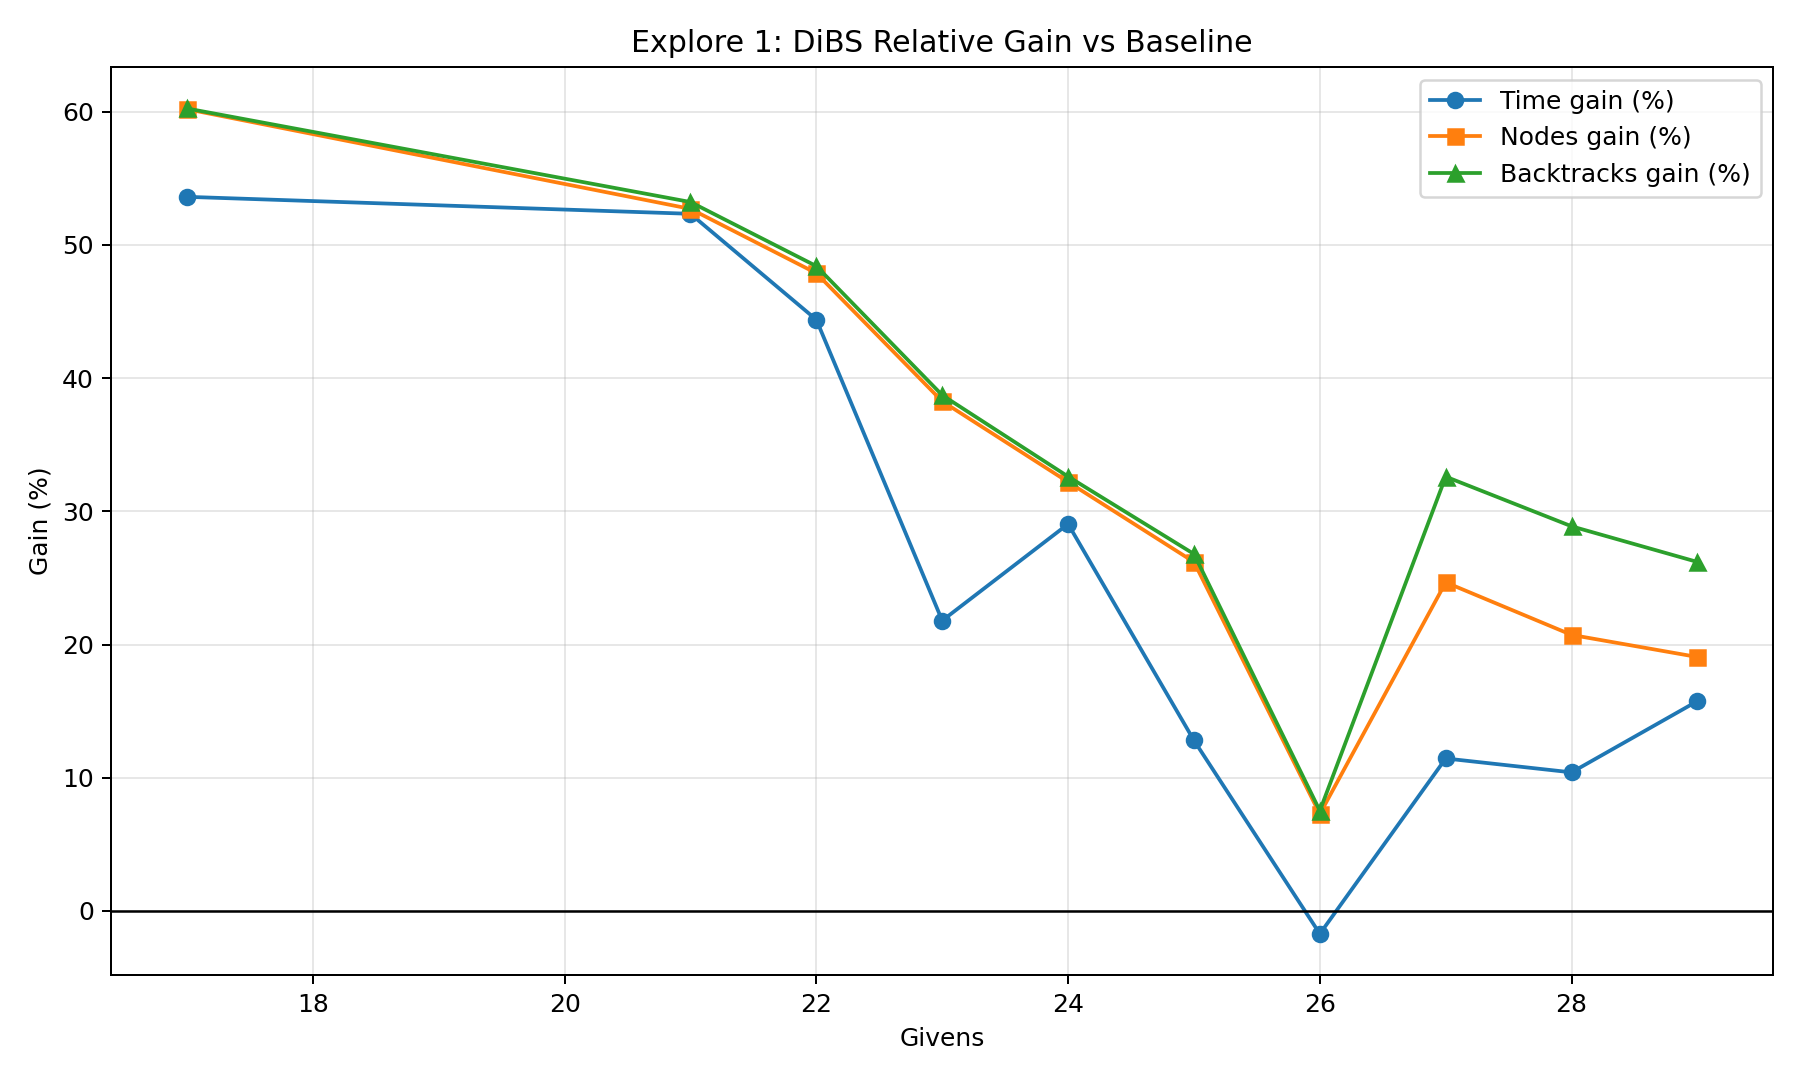
\includegraphics[width=\linewidth]{figures/exp1_gain_curves.png}
\caption{DiBS relative gain over MRV+FC+LCV across puzzle difficulty (measured by givens).}
\label{fig:exp1_gain_curves}
\end{figure}

\textbf{Difficulty-dependent gains.} Figure~\ref{fig:exp1_gain_curves} shows that the advantage of DiBS grows systematically as puzzles become harder.
In the hardest buckets with 17--21 givens, the reductions in time, nodes, and backtracks are consistently in the 40\%--60\% range.
As the number of givens increases, the gains become smaller.
In the easier 25--29-givens buckets, the reductions in nodes and backtracks are mostly around 20\%--30\%, while the time gain becomes visibly weaker and more unstable.
Therefore, the empirical pattern is not a uniform offset across all instances.
Instead, DiBS becomes more valuable exactly when the puzzle difficulty makes branch ordering matter most.

This result is directly aligned with our theoretical analysis.
When a puzzle has fewer givens, propagation is weaker and search must rely more heavily on branching.
Under this regime, an early wrong value choice is more likely to open a deep failing subtree whose cost dominates the overall runtime.
In the decomposition developed in Section~\ref{sec:method}, this means that the leverage of improving the good-first probability becomes larger on harder puzzles because the cost of the wrong subtree is larger.
DiBS is designed precisely for this regime: it uses the diffusion model to improve value ordering at those high-leverage states.
Therefore, the stronger gains on harder buckets are not incidental; they are exactly the behavior the method is supposed to produce.

This figure also clarifies why DiBS should not be judged only by aggregate runtime averages.
On easier puzzles, strong symbolic heuristics already solve most instances with relatively shallow search, so there is limited room for any learned ordering signal to help.
On harder puzzles, however, the tail of the search tree becomes the real bottleneck, and that is where DiBS shows its clearest benefit.
The difficulty analysis provides an external validation of our main claim: DiBS is especially effective on the instances where long-tail search cost is actually generated.



\subsection{DiBS vs. Denoising Steps}

\begin{figure}[h]
\centering
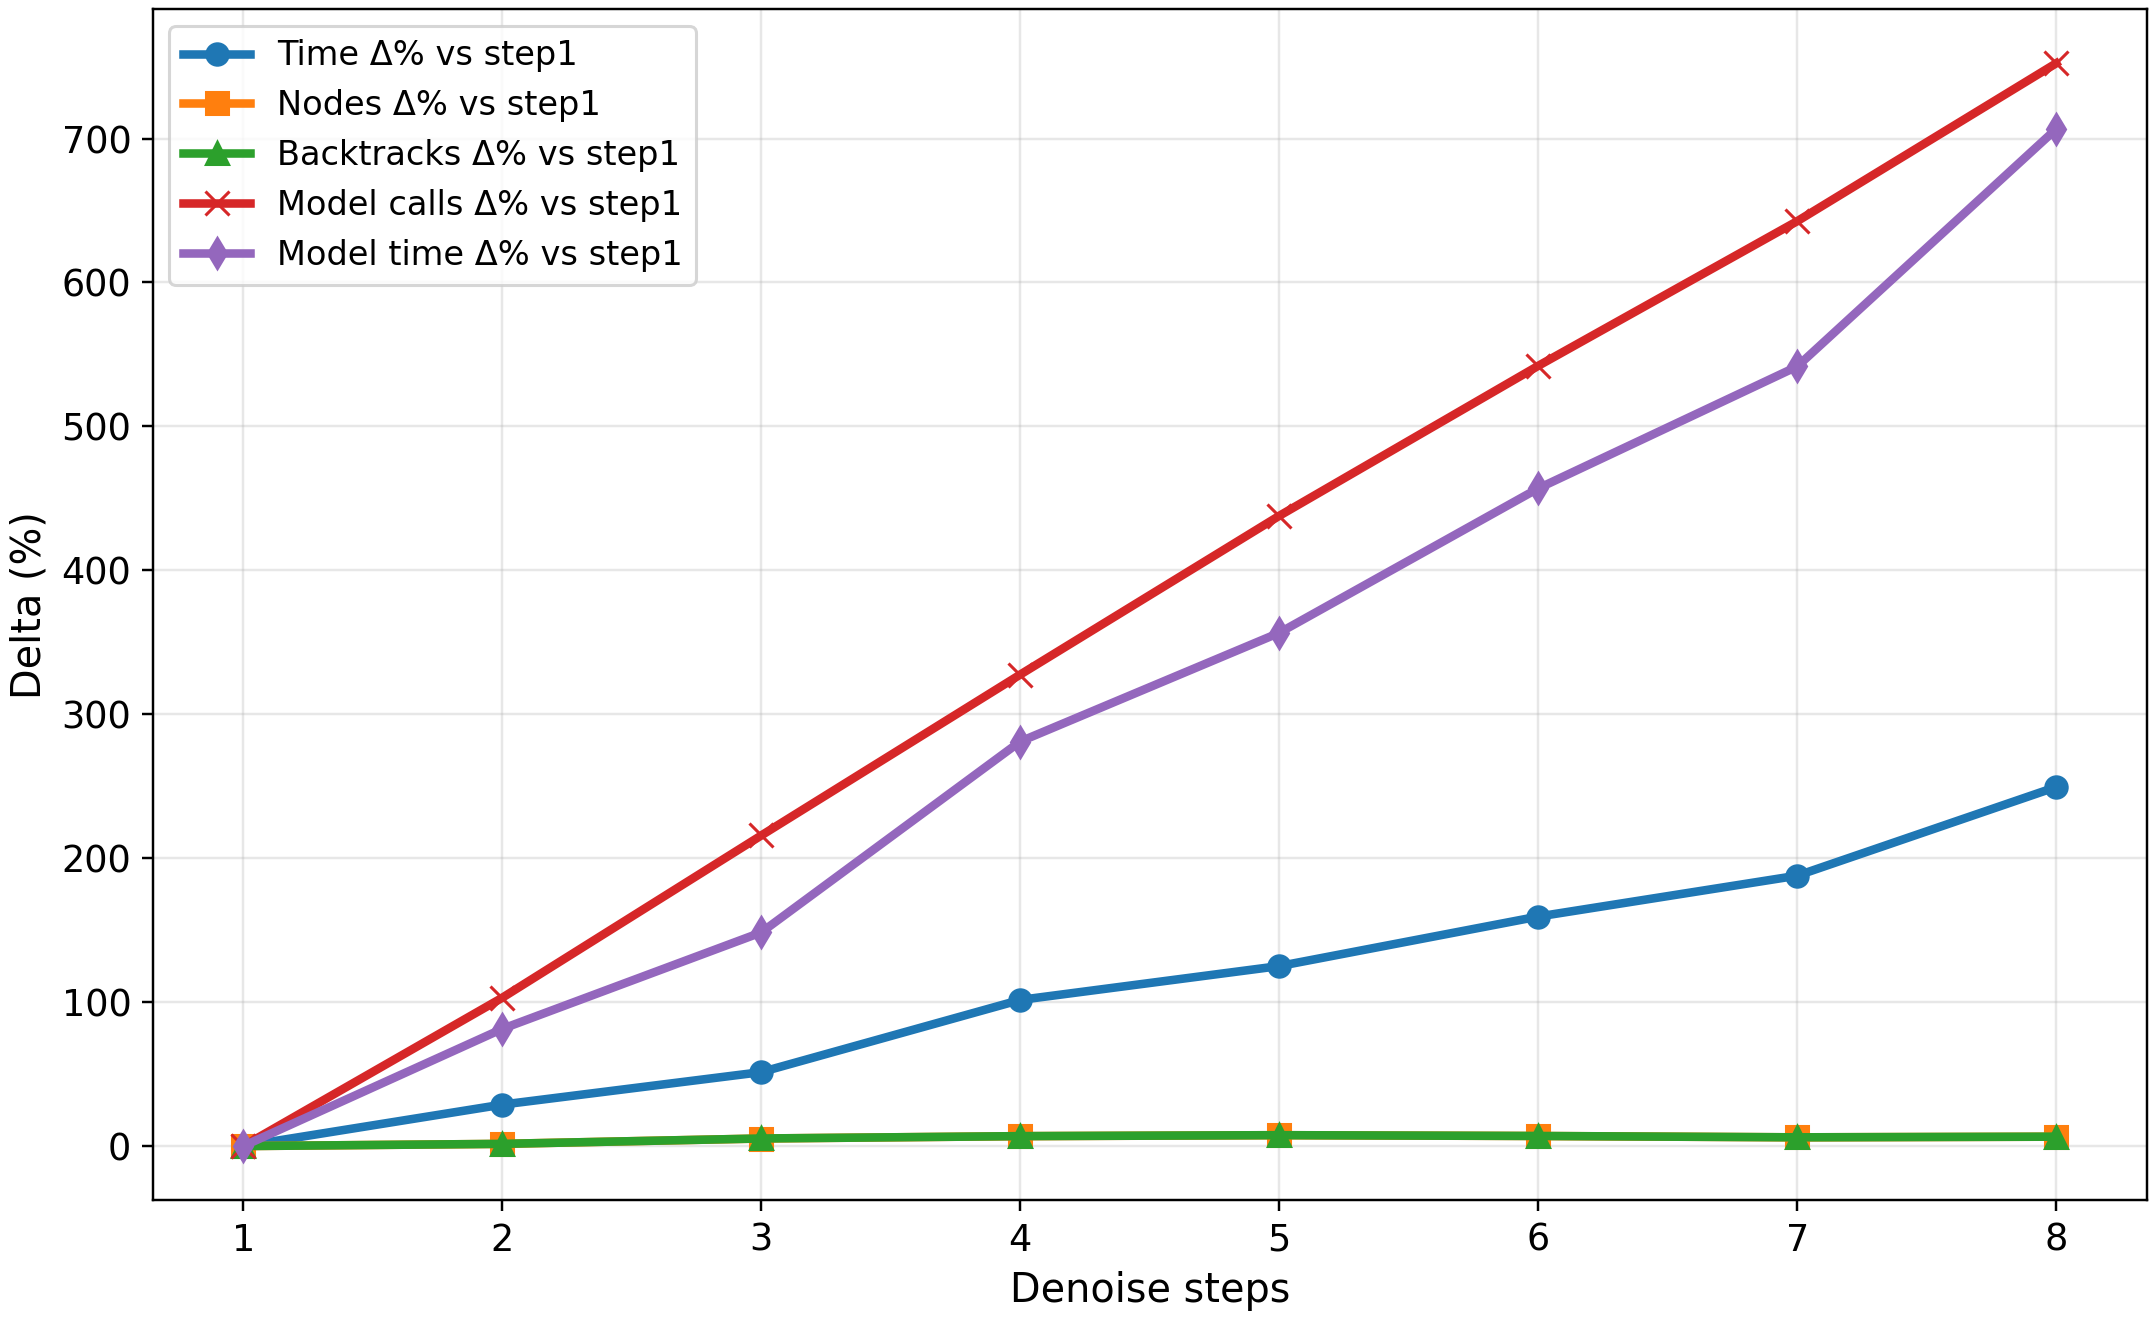
\includegraphics[width=\linewidth]{figures/exp2_steps_deltas_zoom.png}
\caption{Relative change against step=1 over denoising steps 1--8. End-to-end time and model-inference cost increase rapidly as the number of denoising steps grows, whereas nodes and backtracks vary only mildly and provide no compensating search-side reduction.}
\label{fig:steps_delta_zoom}
\end{figure}

\textbf{Global efficiency trend.}
We analyze the denoising-step hyperparameter of DiBS using the Explore-2 setting with 5{,}000 Royle17 instances and steps \(1\) through \(8\).
In this setting, the solved rate is saturated and therefore is not the informative metric; the meaningful comparison lies in search cost and compute cost.
As shown in Fig.~\ref{fig:steps_delta_zoom}, increasing the number of denoising steps consistently worsens overall efficiency under the current solver interface.
Relative to step=1, step=2 already increases time by 28.83\%, nodes by 1.53\%, and backtracks by 1.54\%, while model time increases by 81.44\%.
As the step number further increases, the runtime degradation becomes much larger: at step=4 and step=8, the time deterioration reaches 101.56\% and 249.48\%, respectively.
The intermediate steps follow the same pattern: model-side cost grows rapidly, while the search-side metrics remain within a much smaller range and do not show a compensating reduction.
Therefore, additional denoising does change the model output, but it does not improve the final search trajectory.

This observation is important from the perspective of our theory.
In DiBS, the diffusion model is not used to generate a full Sudoku board.
It is used only to rank a small number of candidate values at a binary branching state.
For this interface, the relevant quantity is not whether the model becomes sharper or more confident after extra denoising, but whether the changed ranking improves the probability of trying the solution-leading branch first strongly enough to amortize the extra inference time.
The results show that this does not happen here.
Step=1 already captures most of the useful global signal needed for branch ordering, and larger steps are a computational burden.

\begin{figure}[!htbp]
\centering

\subfloat[Confidence over unknown cells across steps\label{fig:steps_logits_conf}]{
    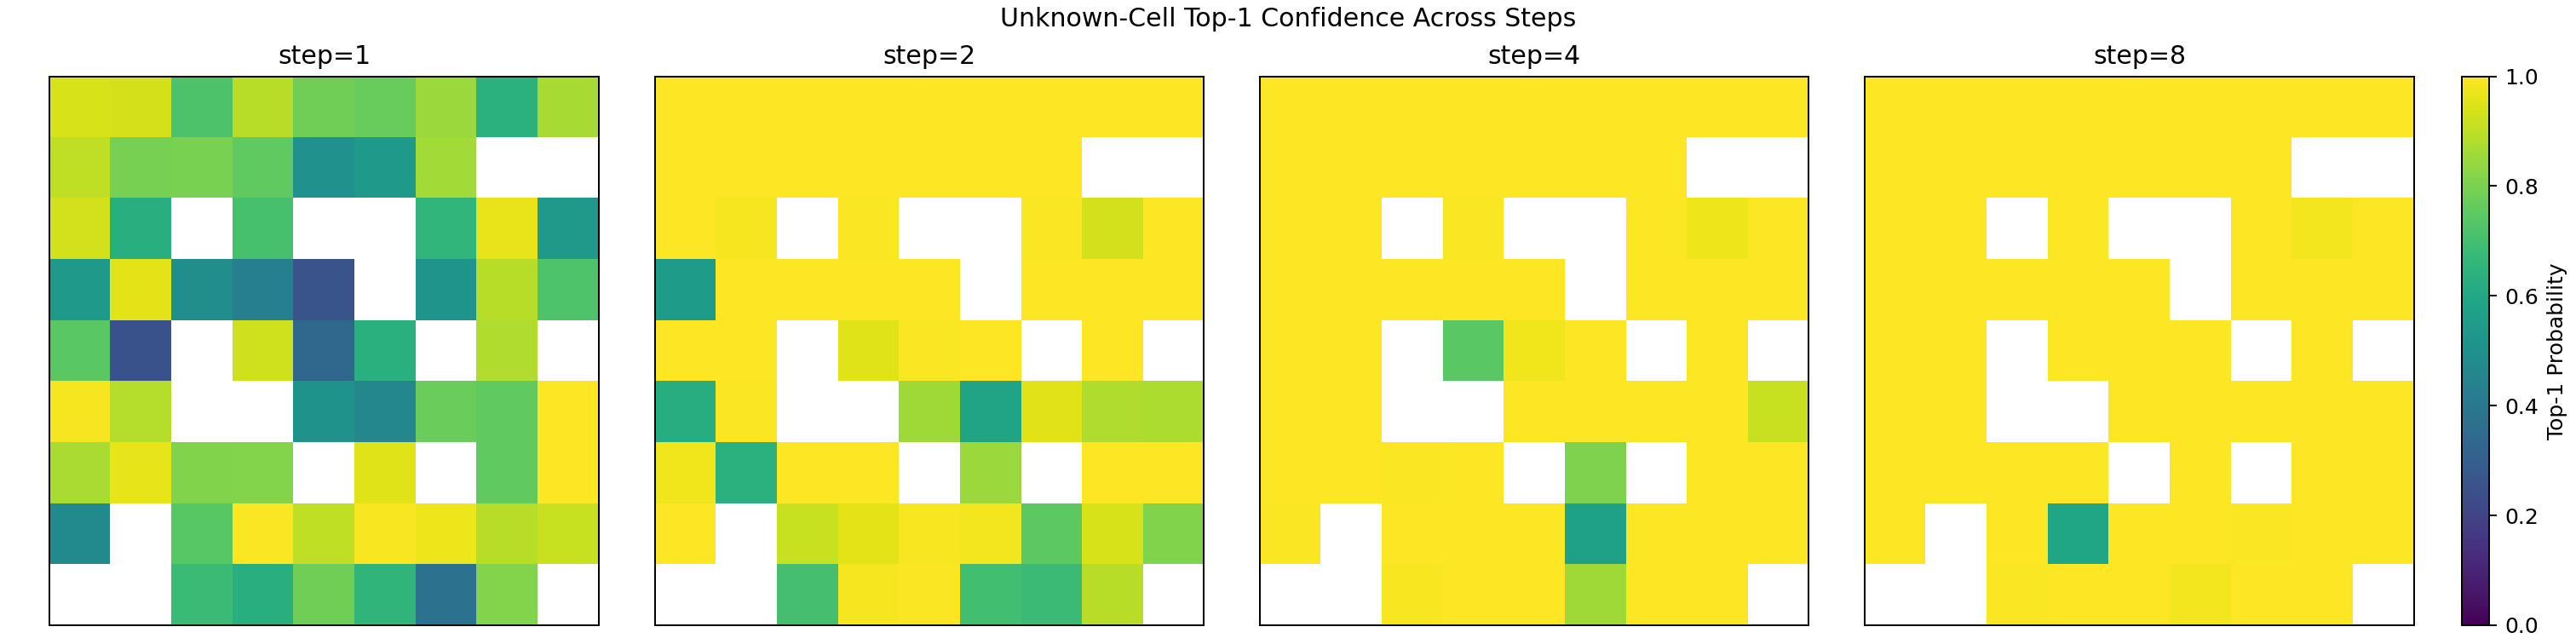
\includegraphics[width=0.9\linewidth]{figures/exp2_logits_top1_confidence.png}
}

\subfloat[Ranking changes vs. step=1 at matched call states\label{fig:steps_logits_betterworse}]{
    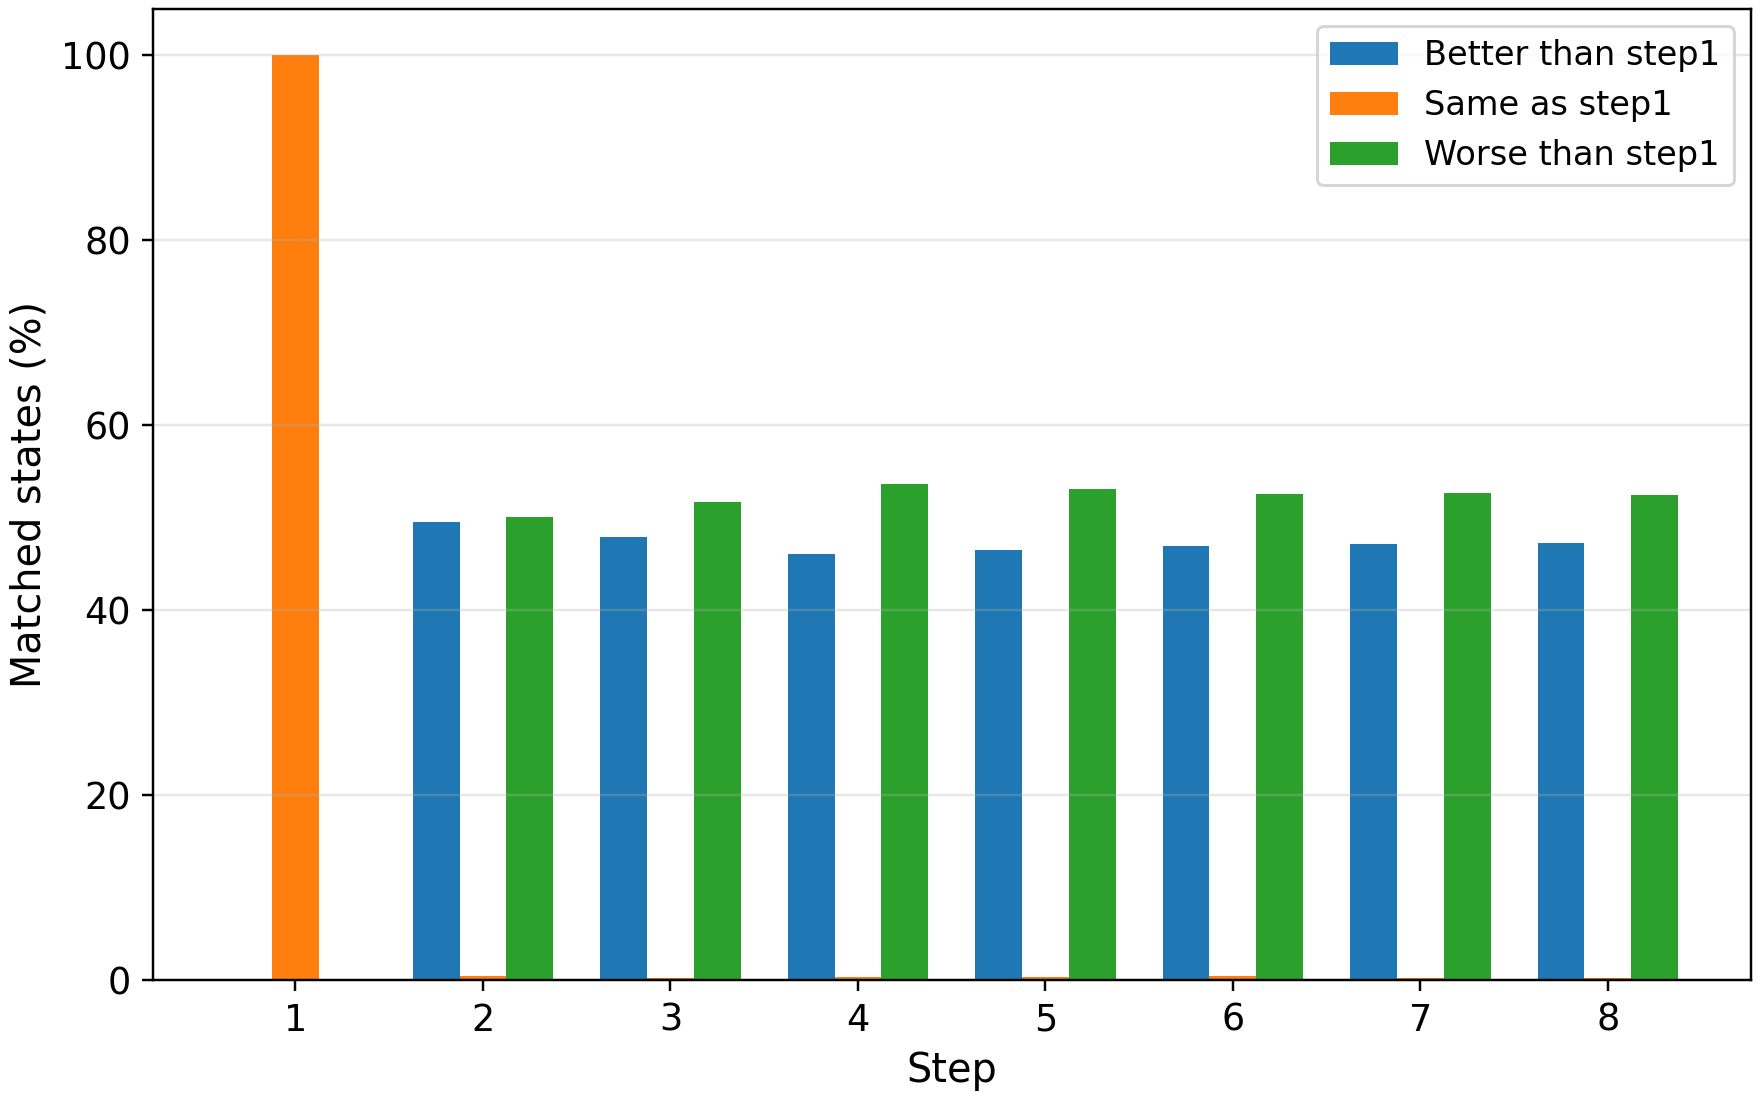
\includegraphics[width=0.9\linewidth]{figures/exp2_callsite_better_worse.png}
}

\subfloat[Call-site top-1 ranking quality across steps\label{fig:steps_logits_quality}]{
    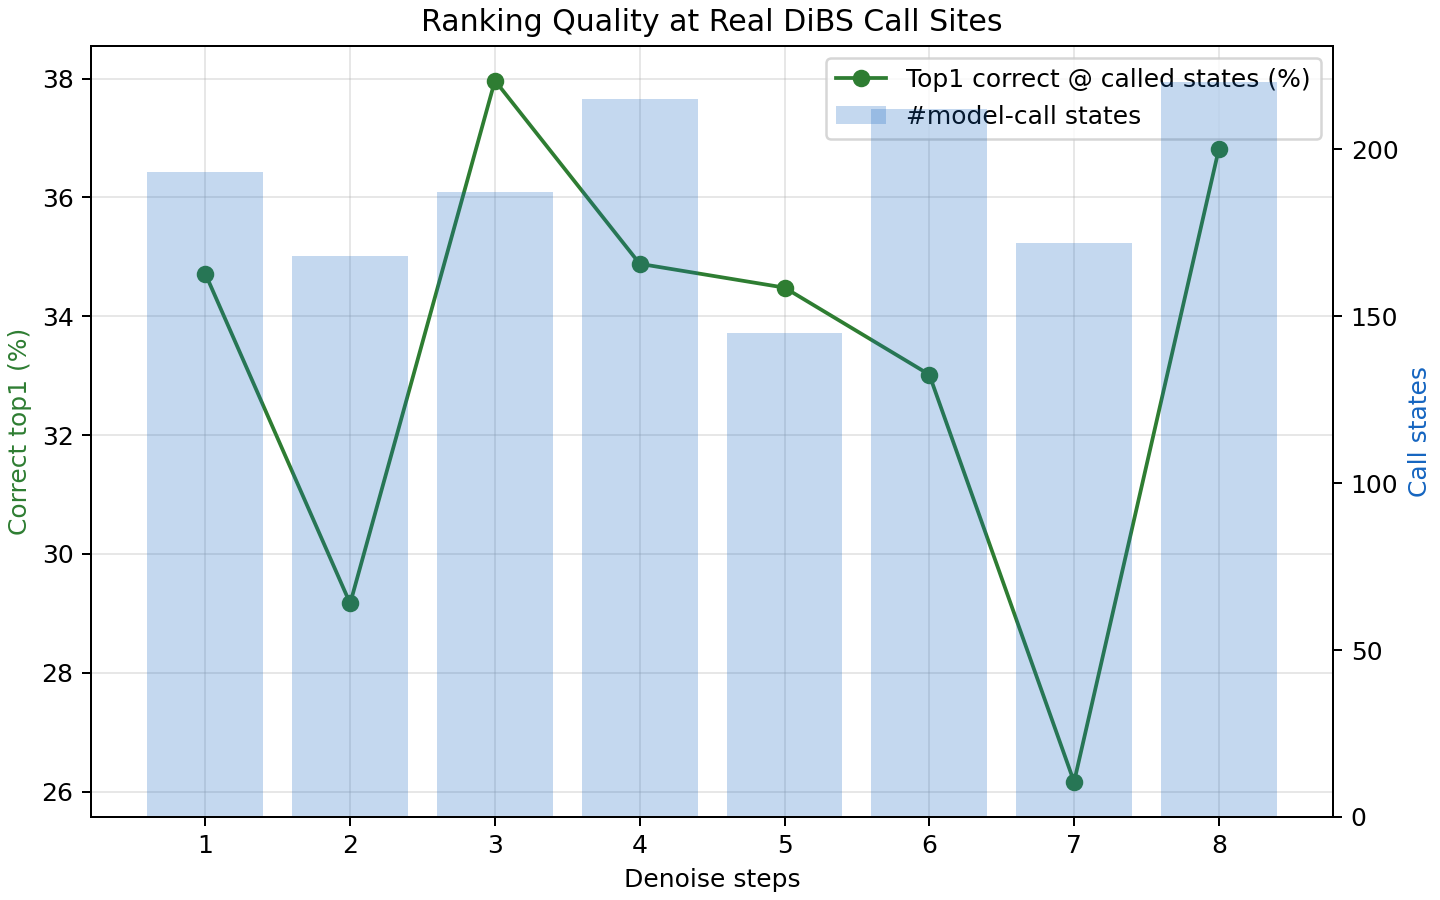
\includegraphics[width=0.9\linewidth]{figures/exp2_callsite_top1_quality.png}
}

\caption{Representative call-state visualization for Explore-2 with denoising steps 1--8.
(a) Different denoising steps produce different confidence landscapes.
(b) Compared with step=1, larger steps introduce both better and worse ranking changes at matched call states, rather than a consistently positive update.
(c) Call-site top-1 quality varies non-monotonically across steps, showing that local ranking quality alone is insufficient to guarantee better global search efficiency.}
\label{fig:steps_logits_case}
\end{figure}

\textbf{Mechanistic explanation.}
The call-state visualizations further explain why more denoising steps do not improve solver efficiency.
In Fig.~\ref{fig:steps_logits_case}(a), larger steps indeed produce sharper confidence maps over unknown cells.
However, sharper confidence is not equivalent to better branch ordering.
In Fig.~\ref{fig:steps_logits_case}(b), the matched-call comparison against step=1 shows both better and worse ranking changes across steps 2--8, rather than a stable improvement in the direction needed by the solver.
In Fig.~\ref{fig:steps_logits_case}(c), the call-site top-1 quality also fluctuates across steps instead of improving monotonically.
Although some larger-step settings can improve local top-1 ranking quality at certain call sites, this local improvement does not reliably translate into lower global search cost.
This is fully consistent with our framework: search efficiency depends on the downstream cost of wrong branches, not on confidence or local ranking quality alone.

Therefore, under the current DiBS integration, the default one-step call is not a weak approximation but the best operating point.
It retains the useful global prior provided by the diffusion model while keeping inference overhead low enough for those gains to convert into real solver efficiency.
This result strengthens the overall message of the paper: for exact search guidance, the best learned component is not necessarily the strongest standalone generator, but the one whose cost-quality trade-off is best matched to the solver interface.


\subsection{DiBS vs. other CSPs}

\begin{table}[t]
\centering
\caption{Generalization of DiBS to satisfiable 3-SAT instances. Nodes and Bkts denote search nodes and backtracks. All methods solve all 1{,}000 test instances for each task. Lower is better.}
\label{tab:other_csps}
\scriptsize
\setlength{\tabcolsep}{2.5pt}
\renewcommand{\arraystretch}{1.06}
\resizebox{\linewidth}{!}{%
\begin{tabular}{llrrrrr}
\toprule
\textbf{Task} & \textbf{Solver} & \textbf{T p95} & \textbf{Nodes} & \textbf{Bkts} & \textbf{Nodes p95} & \textbf{Bkts p95} \\
\midrule
3sat5 & PySAT (Glucose4)~\cite{ignatiev2018pysat,audemard2009glucose} & 0.06 & 5.11 & 1.56 & 6 & 3 \\
 & CP+First+True~\cite{haralick1980increasing} & 0.20 & 5.14 & 2.07 & 7 & 4 \\
 & CP+MRV+True~\cite{freuder1982sufficient} & 0.26 & 5.04 & 1.97 & 7 & 4 \\
 & CP+MRV+JW~\cite{jeroslow1990sat} & 0.33 & \textbf{3.52} & \textbf{0.45} & 6 & 3 \\
 & DiBS & 5.61 & 3.81 & 0.73 & 6 & 3 \\
\midrule
3sat7 & PySAT (Glucose4) & 0.07 & 5.96 & 1.98 & 8 & 4 \\
 & CP+First+True & 0.30 & 6.23 & 2.58 & 10 & 6 \\
 & CP+MRV+True & 0.40 & 5.96 & 2.41 & 10 & 6 \\
 & CP+MRV+JW & 0.51 & 4.69 & \textbf{1.12} & 8 & 5 \\
 & DiBS & 8.50 & \textbf{4.65} & 1.19 & 8 & 5 \\
\midrule
3sat9 & PySAT (Glucose4) & 0.11 & 6.71 & 2.31 & 10 & 5 \\
 & CP+First+True & 0.52 & 7.92 & 3.57 & 14 & 9 \\
 & CP+MRV+True & 0.66 & 7.18 & 2.98 & 12 & 8 \\
 & CP+MRV+JW & 0.83 & 5.95 & 1.66 & 11 & 6 \\
 & DiBS & 13.53 & \textbf{5.88} & \textbf{1.66} & 10 & 6 \\
\bottomrule
\end{tabular}
}
\end{table}

\textbf{SAT as another CSP.} Boolean satisfiability (SAT) is the problem of deciding whether a Boolean formula can be satisfied. For 3-SAT, an instance can be written as
\begin{equation}
	\Phi(z)=\bigwedge_{j=1}^{m} C_j,\qquad
	C_j=(\ell_{j1}\vee \ell_{j2}\vee \ell_{j3}),
	\label{eq:sat_def}
\end{equation}
where \(z=(z_1,\dots,z_n)\in\{0,1\}^n\), and each literal \(\ell_{jk}\) is either \(z_i\) or \(\neg z_i\). The goal is to find an assignment \(a\in\{0,1\}^n\) such that \(\Phi(a)=1\). This is a canonical CSP with Boolean variables and clause constraints \cite{biere2009sat,biere2021sat2}. Standard SAT solving is commonly based on complete backtracking enhanced with Boolean propagation, conflict analysis, and clause learning. In Table~\ref{tab:other_csps}, PySAT is the Python SAT-solver interface, and Glucose4 is the CDCL solver used through it. The label \textit{True} means a fixed value-ordering rule that tries \(z_i=\mathrm{True}\) before \(z_i=\mathrm{False}\). The label \textit{JW} denotes the Jeroslow-Wang literal score
\begin{equation}
	J(\ell)=\sum_{C\in\mathcal{U}(s):\,\ell\in C}2^{-|C_s|},
	\label{eq:jw_score}
\end{equation}
where \(\mathcal{U}(s)\) is the set of unresolved clauses at state \(s\), and \(|C_s|\) is the number of currently unassigned literals in clause \(C\). A larger \(J(\ell)\) gives higher priority to assigning the corresponding literal to true.

\textbf{DiBS adaptation to SAT.} The SAT version of DiBS keeps the same core logic as the Sudoku version: it only changes branch ordering. At a search state \(s=(a,\Phi)\), the symbolic solver first selects a Boolean variable \(z_i\) using the same complete search backbone. The two candidate branches are
\[
	b^+:\ z_i=\mathrm{True},\qquad b^-:\ z_i=\mathrm{False}.
\]
We encode the clause formula and the current partial assignment as a masked token sequence \(E(s)\), where assigned variables are represented by their positive or negative literal tokens and unassigned variables are masked. A SAT-trained MDM then produces logits for the two literal tokens of \(z_i\). DiBS uses
\begin{equation}
	\begin{aligned}
		\mathrm{Score}_\theta(s,b^+) &= \ell_\theta(z_i\mid E(s)),\\
		\mathrm{Score}_\theta(s,b^-) &= \ell_\theta(\neg z_i\mid E(s)),
	\end{aligned}
	\label{eq:sat_dibs_score}
\end{equation}
and explores the higher-scoring branch first. The model is called only when the selected unresolved clause has at most two open literals. All candidates are still explored if needed, so unit propagation, backtracking, and completeness are unchanged.

\textbf{Results.} Table~\ref{tab:other_csps} shows that DiBS solves all 3-SAT test instances and consistently reduces search cost relative to the True-ordering baselines. More importantly, its advantage becomes clearer as the number of SAT variables increases. On 3sat5, DiBS is already much better than CP+MRV+True but still behind the SAT-specific JW rule in average nodes and backtracks. On 3sat7, DiBS reaches the best mean nodes while remaining close to JW in backtracks and matching its p95 search cost. On 3sat9, DiBS becomes the strongest search-cost method in mean nodes, ties the best mean backtracks, and improves the p95 node count over JW. Thus, the learned ordering signal is not merely improving a weak baseline; it becomes competitive with a strong handcrafted SAT value heuristic as the search problem becomes larger.

The wall-clock results should be interpreted separately from the search-cost results. DiBS makes 1.19, 1.79, and 2.50 model calls on average for 3sat5, 3sat7, and 3sat9, with average model times of 4.13 ms, 4.70 ms, and 6.58 ms. Because these formulas are very small, this inference cost dominates runtime, so PySAT/Glucose4 and the symbolic heuristics are faster in milliseconds. This does not contradict the branch-ordering result: PySAT/Glucose4 is a highly optimized CDCL solver, while our SAT DiBS variant intentionally uses a simple complete backbone to isolate the effect of learned value ordering.

\textbf{Interpretation.} These results close the empirical loop with our theory and the puzzle-difficulty discussion. Theorems~\ref{thm:binary_cost} and~\ref{thm:optimal_guidance} show that the value of a better branch order scales with \(\Delta p_s\cdot T(s_w)\), where \(T(s_w)\) is the cost of the failing branch that would be explored after a wrong first choice. Increasing the number of SAT variables enlarges the space in which a wrong literal choice can remain locally consistent before contradiction, so the potential wrong-subtree cost becomes larger. This is the same mechanism observed in Fig.~\ref{fig:exp1_gain_curves}: DiBS is most useful when the instance becomes hard enough for branch ordering to matter. Therefore, the 3-SAT experiment supports the broader claim that DiBS is not tied to Sudoku-specific structure. Once the problem admits a complete branching solver and a learned model can score candidate values under a partial assignment, the same diffusion-informed branch-selection principle can reduce symbolic search while preserving completeness.


%题目难度和优势大小的关系
%关于模型的调用，去噪几步，步数 时间 收益 trade-off
%不能真讲limitation

\section{Conclusion}

In this paper, we introduced \textbf{DiBS}, a diffusion-informed branch-selection method that improves exact Sudoku solving by injecting learned guidance into a complete CP+MRV solver. The key idea is not to replace symbolic search or directly generate full solutions, but to use diffusion-model preferences to improve branch ordering at high-leverage decision points while preserving completeness. This directly targets the long-tail inefficiency of backtracking, where a few wrong early choices can induce large failing subtrees. We also provided a theoretical account of this mechanism. At the local level, our analysis shows that the expected benefit of better branch ordering scales with the cost of the wrong subtree. At the global level, we derived an expected-complexity view in which runtime decomposes into solution-path cost, model-inference overhead, and posterior-weighted wrong-subtree cost, making explicit how model capability enters the final trade-off. Future work should therefore focus on improving the efficiency and scope of guidance. Promising directions include reducing model-call cost, learning cheaper branch-ranking surrogates, extending guidance beyond binary MRV states, and applying the same framework to broader classes of CSPs and exact combinatorial search problems. More broadly, we believe DiBS suggests a useful paradigm for integrating modern generative models with exact symbolic solvers: not by replacing algorithmic structure, but by selectively improving the decisions that matter most.

\bibliographystyle{IEEEtran}
\bibliography{sample-base.bib}


\begin{IEEEbiography}[{\includegraphics[width=1in,height=1.25in,clip,keepaspectratio]{Author photo/Bo Liu}}]{Bo Liu}(Graduate Student Member, IEEE)
is currently pursuing a B.S. degree in Statistics at the School of Mathematics, Jilin University. He's about to join the School of Artificial Intelligence, The Chinese University of Hong Kong, Shenzhen. His research interests include Data Mining, AI4Sci, Computer Vision and LLM. He has published some papers in IEEE International Conference on Acoustics, Speech, and Signal Processing (I-CASSP) and Computer Networks.
\end{IEEEbiography}

\begin{IEEEbiography}[{\includegraphics[width=1in,height=1.25in,clip,keepaspectratio]{Author photo/Yuan Xie.jpg}}]{Yuan Xie}
is currently pursuing the Ph.D. degree in the School of Data Science from The Chinese University of Hong Kong, Shenzhen, China. He received the B.S. degree in Math and Statistics from Xi'an Jiao Tong University, Xi'an, China, in 2022. His research interests include pattern recognition, deep learning, computer vision and image processing. He has published some journal papers in IEEE Transactions on Image Processing (T-IP), IEEE Transactions on Multimedia (T-MM), Knowledge-Based Systems (KBS), and Expert Systems with Applications (ESWA).
\end{IEEEbiography}

\begin{IEEEbiography}[{\includegraphics[width=1in,height=1.25in,clip,keepaspectratio]{Author photo/Yuan Gao.jpg}}]{Yuan Gao}
is currently a PhD candidate at The Chinese University of Hong Kong, Shenzhen. He received the B.Sc. degree from Budapest University of Technology and Economics. Budapest, Hungary, in 2023. His current research interests include breath analysis, signal processing, and machine learning. He has published paper in IEEE Transactions on Consumer Electronics (T-CE).
\end{IEEEbiography}
%\vspace{-20pt}
\begin{IEEEbiography}[{\includegraphics[width=1in,height=1.25in,clip,keepaspectratio]{Author photo/Xiaolong Luo.jpg}}]{Xiaolong Luo}
is currently pursuing the B.S. degree in information management and information systems with Southwest University, Chongqing, China. He has published research papers in journals including Library Research and Biomedical Data Science. His current research interests include recommendation systems and graph neural networks (GNNs), with a focus on graph contrastive learning and ranking optimization.
\end{IEEEbiography}
%\vspace{-20pt}
\begin{IEEEbiography}[{\includegraphics[width=1in,height=1.25in,clip,keepaspectratio]{Author photo/Peng Ye.jpg}}]{Peng Ye}
is currently a Postdoctoral Researcher Fellow at The Chinese University of Hong Kong. He received the Ph.D. degree from Fudan University, Shanghai, China. His research interests include computer vision, network design and optimization. He has published papers in leading journals and conferences, including T-PAMI, IJCV, T-IP, CVPR Oral, NeurIPS Spotlight, ICML, ICLR, ICCV, ECCV, AAAI Oral, ACM MM Oral, and ICME Best
Student Paper, ICASSP, etc. He serves as a reviewer
in kinds of journals and conferences, including T-PAMI, IJCV, T-MM,
TCSVT, NeurIPS, ICML, ICLR, CVPR, ECCV, ICCV, AAAI, etc.
\end{IEEEbiography}
%\vspace{-20pt}
\begin{IEEEbiography}[{\includegraphics[width=1in,height=1.25in,clip,keepaspectratio]{Author photo/Tao Chen.png}}]{Tao Chen} (Senior Member, IEEE)
received the PhD degree in information engineering from Nanyang
Technological University, Singapore, in 2013. He was
a research scientist with the Institute for Infocomm
Research, A$\ast$STAR, Singapore, from 2013 to 2017,
and a senior scientist with Huawei Singapore
Research Center from 2017 to 2018. He is currently
a professor with the School of Information Science
and Technology, Fudan University, Shanghai, China.
His main research interests include computer vision
and machine learning. He has published more than
70 papers in reputable journals and conferences such as IEEE Transactions
on Pattern Analysis and Machine Intelligence/IEEE Transactions on Image
Processing/CVPR/International Journal of Computer Vision.
\end{IEEEbiography}
%\vspace{-20pt}
\begin{IEEEbiography}[{\includegraphics[width=1in,height=1.25in,clip,keepaspectratio]{Author photo/Fujun Han.png}}]{Fujun Han} (Member, IEEE)
is currently a Postdoctoral Researcher Fellow at The Chinese University of Hong Kong, Shenzhen, China. He received the Ph.D. degree from Southwest University, Chongqing, China. His research interests include Multimodal Large Language Models, Computer Vision, and Autonomous Driving. He has published some papers in leading conferences and journals, \textit{e.g.}, ICLR, NeurIPS, ACM MM (Oral), ACM MM, ICDM, IEEE Transactions on Automation Science and Engineering (T-ASE), IEEE Transactions on Intelligent Vehicles (T-IV), IEEE Transactions on Circuits and Systems for Video Technology (T-CSVT), IEEE Transactions on Geoscience and Remote Sensing (T-GRS), IEEE Transactions on Emerging Topics in Computational Intelligence (T-ETCI), IEEE Journal of Selected Topics in Applied Earth Observations and Remote Sensing (I-JSTARS), IEEE Sensors Journal (I-SJ), and Journal of Cleaner Production (J-CP). Besides, He also serves as a reviewer in some excellent conferences and journals, including ICML, NeurIPS, ICLR, ECCV, AAAI, ACM MM, IEEE T-ASE, etc.
\end{IEEEbiography}


%\newpage
\clearpage

\appendices
\section{Proof of Theorem~\ref{thm:binary_cost}}
\label{sec:proof_binary_cost}

We prove the stated decomposition for a binary branching state $s$.
Let the two children be $s_g$ (good, solution-leading) and $s_w$ (wrong, failing), and
let  $T(s_g)$ and $T(s_w)$ denote the costs of fully exploring their subtrees.
We consider a depth-first backtracking solver that explores the first-chosen branch to completion,
and explores the second branch only if the first branch fails.
This matches Algorithm~\ref{alg:dibs_solver} at a binary branching node.

Let $\pi$ be a branch-ordering policy at state $s$, and define the event
\[
A := \{\pi \text{ explores } s_g \text{ before } s_w\}.
\]
By definition, $\mathbb{P}(A)=p_s(\pi)$.
Let $C_\pi(s)$ be the total cost incurred starting from state $s$ until a solution is found.
Under the unique-solution assumption, the solver finds a solution if and only if it reaches
the good branch $s_g$.
Therefore, conditioned on the ordering event $A$:
\begin{itemize}
	\item If $A$ occurs (good-first), then the solver explores the subtree rooted at $s_g$
	until a solution is found, and never needs to fully explore the wrong subtree. Hence
	\[
	C_\pi(s) = T(s_g) \qquad \text{on } A.
	\]
	\item If $A^c$ occurs (wrong-first), then the solver must exhaust the failing subtree rooted at $s_w$
	before backtracking to try $s_g$, after which it incurs $T(s_g)$ to find the solution. Hence
	\[
	C_\pi(s) = T(s_w) + T(s_g) \qquad \text{on } A^c.
	\]
\end{itemize}
Introduce the indicator $\mathbf{1}_A$. We can write this piecewise definition compactly as
\[
C_\pi(s) = T(s_g) + \mathbf{1}_{A^c}\,T(s_w).
\]
Taking expectations on both sides yields
\[
\mathbb{E}[C_\pi(s)]
=
\mathbb{E}[T(s_g)] + \mathbb{E}\!\left[\mathbf{1}_{A^c}\,T(s_w)\right].
\]
At a fixed state $s$, the randomization of the policy affects only the ordering event $A$.
Since $T(s_w)$ is determined by the instance and the solver dynamics within the subtree once it is entered,
we use the standard conditioning identity:
\[
\mathbb{E}\!\left[\mathbf{1}_{A^c}\,T(s_w)\right]
=
\mathbb{P}(A^c)\,\mathbb{E}[T(s_w)]
=
\bigl(1-p_s(\pi)\bigr)\,\mathbb{E}[T(s_w)].
\]
Combining the above establishes
\[
\mathbb{E}[C_\pi(s)]
=
\mathbb{E}[T(s_g)] + \bigl(1-p_s(\pi)\bigr)\,\mathbb{E}[T(s_w)].
\]
Finally, for two policies $\pi_a,\pi_b$, subtracting their decompositions gives
\[
\mathbb{E}[C_{\pi_a}(s)]-\mathbb{E}[C_{\pi_b}(s)]
=
\bigl(p_s(\pi_b)-p_s(\pi_a)\bigr)\,\mathbb{E}[T(s_w)],
\]
which completes the proof.
\qed

\section{Proof of Theorem~\ref{thm:optimal_guidance}}
\label{sec:proof_optimal_guidance}

We work at a fixed satisfiable binary branching state $s$.
Recall that $\Pi_s$ denotes the class of all branch-ordering policies at $s$ that keep the same symbolic
backbone and differ only in how they order the two candidates in $D_{v^\star(s)}$.
For each $\pi\in\Pi_s$, the quantity $p_s(\pi)$ is the probability that $\pi$ explores the
solution-leading child $s_g$ before the failing child $s_w$.
We also defined
\[
p_s^\star := \sup_{\pi\in\Pi_s} p_s(\pi),
\]
and let $\pi_s^\star\in\Pi_s$ denote any policy attaining this supremum.

We first prove the equivalence in Eq.~\eqref{eq:optimal_equiv}.
By Theorem~\ref{thm:binary_cost}, for every policy $\pi\in\Pi_s$,
\[
\mathbb{E}[C_\pi(s)]
=
\mathbb{E}[T(s_g)]
+
\bigl(1-p_s(\pi)\bigr)\,\mathbb{E}[T(s_w)].
\]
At the fixed state $s$, both $\mathbb{E}[T(s_g)]$ and $\mathbb{E}[T(s_w)]$ are independent of the
choice of policy, and $\mathbb{E}[T(s_w)]\ge 0$.
Therefore $\mathbb{E}[C_\pi(s)]$ is an affine decreasing function of $p_s(\pi)$.
It follows that minimizing $\mathbb{E}[C_\pi(s)]$ over $\Pi_s$ is equivalent to maximizing $p_s(\pi)$ over $\Pi_s$:
\[
\arg\min_{\pi\in\Pi_s}\mathbb{E}[C_\pi(s)]
=
\arg\max_{\pi\in\Pi_s} p_s(\pi).
\]
Since $\pi_s^\star$ attains $p_s^\star$, it belongs to both sets, establishing Eq.~\eqref{eq:optimal_equiv}.

Next, let $\pi\in\Pi_s$ be arbitrary.
Applying Theorem~\ref{thm:binary_cost} once to $\pi$ and once to $\pi_s^\star$, we obtain
\[
\mathbb{E}[C_\pi(s)]
=
\mathbb{E}[T(s_g)]
+
\bigl(1-p_s(\pi)\bigr)\,\mathbb{E}[T(s_w)],
\]
and
\[
\mathbb{E}[C_{\pi_s^\star}(s)]
=
\mathbb{E}[T(s_g)]
+
\bigl(1-p_s(\pi_s^\star)\bigr)\,\mathbb{E}[T(s_w)].
\]
Subtracting the two identities gives
\[
\mathbb{E}[C_\pi(s)]-\mathbb{E}[C_{\pi_s^\star}(s)]
=
\bigl(p_s(\pi_s^\star)-p_s(\pi)\bigr)\,\mathbb{E}[T(s_w)].
\]
By definition of $\pi_s^\star$, we have $p_s(\pi_s^\star)=p_s^\star$, hence
\[
\mathbb{E}[C_\pi(s)]-\mathbb{E}[C_{\pi_s^\star}(s)]
=
\bigl(p_s^\star-p_s(\pi)\bigr)\,\mathbb{E}[T(s_w)],
\]
which is Eq.~\eqref{eq:oracle_gap_general}.

Finally, for DiBS we substitute $\pi=\pi_\theta$ and use the definition
\[
\delta_s(\theta):=p_s^\star-p_s(\pi_\theta).
\]
Therefore,
\[
\mathbb{E}[C_{\pi_\theta}(s)]-\mathbb{E}[C_{\pi_s^\star}(s)]
=
\delta_s(\theta)\,\mathbb{E}[T(s_w)],
\]
which is Eq.~\eqref{eq:oracle_gap_dibs}.
This completes the proof.
\qed

\section{Complete solver with DiBS}

Algorithm~\ref{alg:dibs_solver} presents the complete solver equipped with DiBS. The overall backbone remains standard depth-first search with sound constraint propagation and MRV branching. DiBS only changes the ordering of candidate values, and is activated only when the selected MRV variable has a binary domain.

\begin{algorithm}[h]
	\caption{Complete CP+MRV solver with DiBS branch ordering}
	\label{alg:dibs_solver}
	\begin{algorithmic}[1]
		\Function{Solve}{$x,\{D_v\}_{v\in V}$}
		\State Apply sound constraint propagation to $(x,\{D_v\}_{v\in V})$
		\If{$\exists v\in V$ with $D_v=\varnothing$}
		\State \Return UNSAT
		\EndIf
		\If{$x$ is complete}
		\State \Return $x$
		\EndIf

		\State Choose
		$
		v^\star \in \arg\min_{v:\,x(v)=0}|D_v|
		$
		\State $L \gets$ a default ordering of $D_{v^\star}$

		\If{$|D_{v^\star}| = 2$}
		\State Construct the conditioning grid $C_e(s)$ from the current partial state
		\State Query the diffusion model once on $C_e(s)$
		\ForAll{$d \in D_{v^\star}$}
		\State Compute the diffusion preference score Eq.~\eqref{eq:pref_def}
		\State Compute the peer-consistency term Eq.~\eqref{eq:cons_def}
		\State Compute the final branch score Eq.~\eqref{eq:final_score}
		\EndFor
		\State Reorder $L$ by decreasing final branch score
		\EndIf

		\ForAll{$d \in L$}
		\State Create a child state by assigning $x(v^\star)\gets d$
		\State $r \gets$ \Call{Solve}{child state}
		\If{$r \neq \mathrm{UNSAT}$}
		\State \Return $r$
		\EndIf
		\EndFor

		\State \Return UNSAT
		\EndFunction
	\end{algorithmic}
\end{algorithm}



\section{Global Expected Complexity of DiBS}
\label{sec:global_complexity}

The statewise results in Theorem~\ref{thm:binary_cost} and
Theorem~\ref{thm:optimal_guidance} explain the value of better
branch ordering at a single binary MRV state. We now lift this
view to the whole solving process.

We emphasize that, because DiBS preserves completeness and only
changes branch ordering, it does not alter the worst-case complexity
class of complete backtracking in the absence of additional assumptions.
Therefore, the meaningful object of analysis is the \emph{expected}
solving cost under an instance distribution or, equivalently, under a
probabilistic model of branch-order correctness. For standard
\(9\times 9\) Sudoku, this should be read as an expected-cost statement
over a fixed-size benchmark; asymptotic order statements become
meaningful for generalized Sudoku or CSP families whose size grows.

Consider a satisfiable instance with a unique solution. Let
\(s_1,\dots,s_H\) denote the binary-trigger states on the
solution-leading trajectory, i.e., the MRV states satisfying
\(|D_{v^\star(s_h)}|=2\) that are eventually encountered by the
complete solver. For each triggered state \(s_h\), let \(s_{h,g}\)
and \(s_{h,w}\) denote the solution-leading child and the failing
sibling child, respectively, in the same sense as \(s_g\) and \(s_w\)
in Theorem~\ref{thm:binary_cost}. Define
\[
A_h :=
\{\pi_\theta \text{ explores } s_{h,g}
\text{ before } s_{h,w}\},
\]
and let
\[
p_h(\theta)
:=
p_{s_h}(\pi_\theta)
=
\mathbb{P}(A_h\mid s_h)
\]
be the branch-ordering success probability of DiBS at state \(s_h\).
Let \(T(s_{h,w})\) be the cost of fully exploring the failing sibling
subtree rooted at \(s_{h,w}\), excluding the model call at \(s_h\).
Let \(\tau_h(\theta)\) be the inference cost of the DiBS call at
\(s_h\), and let \(G_H\) denote the cost incurred along the
solution-leading trajectory, excluding all failing sibling subtrees
and excluding the DiBS inference overheads at the \(H\) triggered states.

With this notation, the global analysis below is exactly the pathwise
counterpart of the local decomposition in Theorem~\ref{thm:binary_cost}:
the local term
\[
(1-p_s(\pi))T(s_w)
\]
is accumulated over all triggered binary states as
\[
\sum_{h=1}^{H}
\bigl(1-p_{s_h}(\pi_\theta)\bigr)T(s_{h,w}).
\]

\begin{theorem}[Global posterior-weighted cost decomposition]
	\label{thm:global_cost}
	For a satisfiable instance with a unique solution, the total solving
	cost of DiBS satisfies
	\begin{equation}
		C_{\pi_\theta}
		=
		G_H
		+
		\sum_{h=1}^{H} \tau_h(\theta)
		+
		\sum_{h=1}^{H}
		\mathbf{1}_{A_h^c}\, T(s_{h,w}).
		\label{eq:global_pathwise}
	\end{equation}
	Consequently,
	\begin{equation}
		\mathbb{E}[C_{\pi_\theta}]
		=
		\mathbb{E}[G_H]
		+
		\sum_{h=1}^{H} \mathbb{E}[\tau_h(\theta)]
		+
		\sum_{h=1}^{H}
		\mathbb{E}\!\left[
		\bigl(1-p_{s_h}(\pi_\theta)\bigr) T(s_{h,w})
		\right].
		\label{eq:global_expectation}
	\end{equation}
	If \(p_{s_h}(\pi_\theta)\), \(T(s_{h,w})\), and \(\tau_h(\theta)\)
	are treated as deterministic conditional on the instance, then
	Eq.~\eqref{eq:global_expectation} reduces to
	\begin{equation}
		\mathbb{E}[C_{\pi_\theta}\mid \mathcal{I}]
		=
		G_H
		+
		\sum_{h=1}^{H} \tau_h(\theta)
		+
		\sum_{h=1}^{H}
		\bigl(1-p_{s_h}(\pi_\theta)\bigr)T(s_{h,w}).
		\label{eq:global_expectation_fixed_instance}
	\end{equation}
\end{theorem}

\begin{proof}
	For each triggered state \(s_h\), define the mistake indicator
	\[
	M_h := \mathbf{1}_{A_h^c}.
	\]
	Because the solver is complete and the instance is satisfiable with
	a unique solution, every state \(s_h\) on the solution-leading
	trajectory is eventually reached, regardless of whether earlier states
	make temporary wrong-first decisions. Moreover, the failing sibling
	subtrees attached to distinct states \(s_h\) are disjoint, and each
	such subtree is explored at most once.

	Therefore, the total solving cost decomposes pathwise as
	\[
	C_{\pi_\theta}
	=
	G_H
	+
	\sum_{h=1}^{H} \tau_h(\theta)
	+
	\sum_{h=1}^{H} M_h T(s_{h,w}),
	\]
	which is Eq.~\eqref{eq:global_pathwise}. Taking expectations gives
	\[
	\mathbb{E}[C_{\pi_\theta}]
	=
	\mathbb{E}[G_H]
	+
	\sum_{h=1}^{H}\mathbb{E}[\tau_h(\theta)]
	+
	\sum_{h=1}^{H}\mathbb{E}[M_h T(s_{h,w})].
	\]
	Using \(M_h=\mathbf{1}_{A_h^c}\) and
	\[
	\mathbb{P}(A_h^c\mid s_h)
	=
	1-p_{s_h}(\pi_\theta),
	\]
	we obtain
	\[
	\mathbb{E}[M_h T(s_{h,w})]
	=
	\mathbb{E}\!\left[
	\bigl(1-p_{s_h}(\pi_\theta)\bigr)T(s_{h,w})
	\right],
	\]
	which proves Eq.~\eqref{eq:global_expectation}. The fixed-instance
	form in Eq.~\eqref{eq:global_expectation_fixed_instance} follows
	immediately when \(p_{s_h}(\pi_\theta)\), \(T(s_{h,w})\), and
	\(\tau_h(\theta)\) are treated as deterministic conditional on the
	instance.
\end{proof}

Theorem~\ref{thm:global_cost} makes the global mechanism of DiBS
explicit. The total cost consists of three parts:The first term, \(G_H\), is contributed by the symbolic backbone along
the solution-leading trajectory. The second term,
\(\sum_h \tau_h(\theta)\), is the price paid for querying the diffusion
model. The third term,
\[
\sum_{h=1}^{H}
\bigl(1-p_{s_h}(\pi_\theta)\bigr)T(s_{h,w}),
\]
is the expected search waste caused by trying the failing sibling branch
first. Thus, DiBS is beneficial not simply when the model is confident,
but when it reduces the probability of wrong-first ordering on states
whose failing sibling subtree \(T(s_{h,w})\) is large. This is the global
version of the leverage term in Theorem~\ref{thm:binary_cost}.

We next derive a capability-dependent bound. Let
\(\rho_{\theta,H}\in[0,1]\) denote a lower bound on the DiBS
branch-ordering success probability over the \(H\) triggered states:
\[
p_{s_h}(\pi_\theta)\ge \rho_{\theta,H},
\qquad h=1,\dots,H.
\]
This quantity summarizes the model capability at the exact interface
used by DiBS. A stronger model corresponds to a larger
\(\rho_{\theta,H}\), or equivalently a smaller branch-ordering error
\(1-\rho_{\theta,H}\).

\begin{theorem}[Capability-dependent global complexity bound]
	\label{thm:capability_bound}
	Suppose that for all triggered states on the solution-leading trajectory:
	\begin{enumerate}
		\item \(p_{s_h}(\pi_\theta)\ge \rho_{\theta,H}\);
		\item \(\tau_h(\theta)\le \bar{\tau}_{\theta,H}\);
		\item \(T(s_{h,w}) \le c\, b^{H-h}\) for some constants \(c>0\)
		and \(b>1\).
	\end{enumerate}
	Then
	\begin{equation}
		\mathbb{E}[C_{\pi_\theta}\mid \mathcal{I}]
		\le
		G_H
		+
		H\bar{\tau}_{\theta,H}
		+
		c(1-\rho_{\theta,H})
		\sum_{h=1}^{H} b^{H-h}.
		\label{eq:capability_bound_pre}
	\end{equation}
	In particular,
	\begin{equation}
		\mathbb{E}[C_{\pi_\theta}\mid \mathcal{I}]
		=
		O\!\Big(
		G_H
		+
		H\bar{\tau}_{\theta,H}
		+
		(1-\rho_{\theta,H})\, b^H
		\Big).
		\label{eq:capability_bound}
	\end{equation}
	If, in addition, the cost of advancing one step along the
	solution-leading trajectory is bounded by \(\kappa_H\), so that
	\(G_H=O(H\kappa_H)\), then
	\begin{equation}
		\mathbb{E}[C_{\pi_\theta}\mid \mathcal{I}]
		=
		O\!\Big(
		H(\kappa_H+\bar{\tau}_{\theta,H})
		+
		(1-\rho_{\theta,H})\, b^H
		\Big).
		\label{eq:capability_bound_with_path}
	\end{equation}
\end{theorem}

\begin{proof}
	Starting from Eq.~\eqref{eq:global_expectation_fixed_instance},
	\[
	\mathbb{E}[C_{\pi_\theta}\mid \mathcal{I}]
	=
	G_H
	+
	\sum_{h=1}^{H} \tau_h(\theta)
	+
	\sum_{h=1}^{H}
	\bigl(1-p_{s_h}(\pi_\theta)\bigr)T(s_{h,w}).
	\]
	By assumptions 1--3,
	\[
	\sum_{h=1}^{H} \tau_h(\theta)
	\le
	H\bar{\tau}_{\theta,H},
	\]
	and
	\[
	\sum_{h=1}^{H}
	\bigl(1-p_{s_h}(\pi_\theta)\bigr)T(s_{h,w})
	\le
	(1-\rho_{\theta,H})
	\sum_{h=1}^{H} c\,b^{H-h}.
	\]
	Substituting these two bounds proves Eq.~\eqref{eq:capability_bound_pre}.
	Since \(\sum_{h=1}^{H} b^{H-h}=O(b^H)\),
	Eq.~\eqref{eq:capability_bound} follows. The final statement is
	obtained by substituting \(G_H=O(H\kappa_H)\).
\end{proof}

The final bound can be read as
\[
\mathbb{E}[C_{\pi_\theta}\mid \mathcal{I}]
=
O\!\Big(
\underbrace{H(\kappa_H+\bar{\tau}_{\theta,H})}_{\text{path plus inference}}
+
\underbrace{(1-\rho_{\theta,H})b^H}_{\text{residual wrong-subtree search}}
\Big).
\]
Thus, the expected cost of DiBS has two qualitatively different parts.
The first part is the cost of moving along the solution-leading trajectory
and paying for model calls. The second part is the exponential search
cost that remains when DiBS ranks a wrong sibling branch first. The model
does not remove this term by pruning; it reduces the multiplier
\(1-\rho_{\theta,H}\), i.e., the probability of making a wrong-first
branching decision at the relevant binary states.

Theorem~\ref{thm:capability_bound} therefore yields a simple complexity
phase diagram. If the model capability does not improve with problem
size, i.e.,
\[
1-\rho_{\theta,H}=\Theta(1),
\]
then the expected runtime remains exponential in \(H\). In this case,
DiBS can still reduce constants or improve practical tail behavior, but
it does not change the exponential nature of complete backtracking.

If the model error decays exponentially,
\[
1-\rho_{\theta,H}=O(b^{-\lambda H}),
\qquad 0<\lambda<1,
\]
then
\[
\mathbb{E}[C_{\pi_\theta}\mid \mathcal{I}]
=
O\!\Big(
H(\kappa_H+\bar{\tau}_{\theta,H})
+
b^{(1-\lambda)H}
\Big).
\]
In this regime, DiBS reduces the effective exponent of the residual
wrong-subtree search from \(H\) to \((1-\lambda)H\).

If the model is strong enough that
\[
1-\rho_{\theta,H}=O(b^{-H}),
\]
then the exponential wrong-subtree term is fully amortized and the
runtime reduces to the path-plus-inference term
\[
\mathbb{E}[C_{\pi_\theta}\mid \mathcal{I}]
=
O\!\big(H(\kappa_H+\bar{\tau}_{\theta,H})\big).
\]

This shows precisely how model capability affects search complexity.
The relevant quantity is not whether the diffusion model can generate a
complete Sudoku solution by itself, but whether its branch-ordering error
\(1-\rho_{\theta,H}\) becomes small enough at high-leverage binary states
to offset the exponential growth of failing-subtree cost.

\paragraph{Empirical-Bayes estimate of model capability.}
A practical way to estimate \(\rho_{\theta,H}\) from validation data is
to treat each called binary state as a Bernoulli trial indicating whether
DiBS ranks the solution-leading child first. Let \(Z_i\in\{0,1\}\) be
this indicator over \(n\) called states, and place a Beta prior
\[
\rho_{\theta,H}\sim \mathrm{Beta}(a_0,b_0),
\qquad
Z_i\mid \rho_{\theta,H}\sim \mathrm{Bernoulli}(\rho_{\theta,H}).
\]
If \(m=\sum_{i=1}^{n} Z_i\), then the posterior is
\[
\rho_{\theta,H}\mid Z_{1:n}
\sim
\mathrm{Beta}(a_0+m,\; b_0+n-m),
\]
with posterior mean
\begin{equation}
	\widehat{\rho}_{\theta,H}
	=
	\frac{a_0+m}{a_0+b_0+n}.
	\label{eq:beta_posterior_mean}
\end{equation}
Substituting \(\widehat{\rho}_{\theta,H}\) into
Eq.~\eqref{eq:capability_bound} gives a data-driven estimate of the
expected search complexity of DiBS. Although this Beta-Bernoulli model
is a simplification, it provides a principled summary of model capability
at the same binary branch-ordering interface analyzed in
Theorem~\ref{thm:binary_cost} and used by DiBS.








\vfill

\end{document}
